% **************************************************************************************************************
% A Classic Thesis Style
% An Homage to The Elements of Typographic Style
%
% Copyright (C) 2018 André Miede and Ivo Pletikosić
%
% If you like the style then I would appreciate a postcard. My address
% can be found in the file ClassicThesis.pdf. A collection of the
% postcards I received so far is available online at
% http://postcards.miede.de
%
% License:
% This program is free software; you can redistribute it and/or modify
% it under the terms of the GNU General Public License as published by
% the Free Software Foundation; either version 2 of the License, or
% (at your option) any later version.
%
% This program is distributed in the hope that it will be useful,
% but WITHOUT ANY WARRANTY; without even the implied warranty of
% MERCHANTABILITY or FITNESS FOR A PARTICULAR PURPOSE.  See the
% GNU General Public License for more details.
%
% You should have received a copy of the GNU General Public License
% along with this program; see the file COPYING.  If not, write to
% the Free Software Foundation, Inc., 59 Temple Place - Suite 330,
% Boston, MA 02111-1307, USA.
%
% PLEASE SEE ALSO THE AUTHORS' NOTE REGARDING THIS LICENSE
% IN THE DOCUMENTATION (ClassicThesis.pdf --> Chapter 1 / Chapter01.tex)
% **************************************************************************************************************
\RequirePackage{silence} % :-\
    \WarningFilter{scrreprt}{Usage of package `titlesec'}
    %\WarningFilter{scrreprt}{Activating an ugly workaround}
    \WarningFilter{titlesec}{Non standard sectioning command detected}
%% Changing the documentclass declaration to fit on one line for texcount
% \documentclass[
%     twoside,
%     openright,
%     titlepage,
%     numbers=noenddot,
%     % 1headlines,
%     headinclude,
%     footinclude,
%     cleardoublepage=empty,
%     abstract=on,
%     BCOR=5mm,
%     paper=letter,
%     fontsize=11pt
% ]{scrreprt}
\documentclass[oneside,titlepage,numbers=noenddot,headinclude,footinclude,abstract=on,BCOR=5mm,paper=letter,fontsize=11pt]{scrreprt}

%********************************************************************
% Note: Make all your adjustments in here
%*******************************************************
% ****************************************************************************************************
% classicthesis-config.tex
% formerly known as loadpackages.sty, classicthesis-ldpkg.sty, and classicthesis-preamble.sty
% Use it at the beginning of your ClassicThesis.tex, or as a LaTeX Preamble
% in your ClassicThesis.{tex,lyx} with % ****************************************************************************************************
% classicthesis-config.tex
% formerly known as loadpackages.sty, classicthesis-ldpkg.sty, and classicthesis-preamble.sty
% Use it at the beginning of your ClassicThesis.tex, or as a LaTeX Preamble
% in your ClassicThesis.{tex,lyx} with % ****************************************************************************************************
% classicthesis-config.tex
% formerly known as loadpackages.sty, classicthesis-ldpkg.sty, and classicthesis-preamble.sty
% Use it at the beginning of your ClassicThesis.tex, or as a LaTeX Preamble
% in your ClassicThesis.{tex,lyx} with \input{classicthesis-config}
% ****************************************************************************************************
% If you like the classicthesis, then I would appreciate a postcard.
% My address can be found in the file ClassicThesis.pdf. A collection
% of the postcards I received so far is available online at
% http://postcards.miede.de
% ****************************************************************************************************


% ****************************************************************************************************
% 0. Set the encoding of your files. UTF-8 is the only sensible encoding nowadays. If you can't read
% äöüßáéçèê∂åëæƒÏ€ then change the encoding setting in your editor, not the line below. If your editor
% does not support utf8 use another editor!
% ****************************************************************************************************
\PassOptionsToPackage{utf8}{inputenc}
  \usepackage{inputenc}

\PassOptionsToPackage{T1}{fontenc} % T2A for cyrillics
  \usepackage{fontenc}


% ****************************************************************************************************
% 1. Configure classicthesis for your needs here, e.g., remove "drafting" below
% in order to deactivate the time-stamp on the pages
% (see ClassicThesis.pdf for more information):
% ****************************************************************************************************
\PassOptionsToPackage{
  drafting=false,    % print version information on the bottom of the pages
  tocaligned=false, % the left column of the toc will be aligned (no indentation)
  dottedtoc=true,  % page numbers in ToC flushed right
  eulerchapternumbers=true, % use AMS Euler for chapter font (otherwise Palatino)
  linedheaders=false,       % chapter headers will have line above and beneath
  floatperchapter=true,     % numbering per chapter for all floats (i.e., Figure 1.1)
  eulermath=false,  % use awesome Euler fonts for mathematical formulae (only with pdfLaTeX)
  beramono=true,    % toggle a nice monospaced font (w/ bold)
  palatino=true,    % deactivate standard font for loading another one, see the last section at the end of this file for suggestions
  style=classicthesis % classicthesis, arsclassica
}{classicthesis}


% ****************************************************************************************************
% 2. Personal data and user ad-hoc commands (insert your own data here)
% ****************************************************************************************************
\newcommand{\myTitle}{The Dubious Benefits of Predictive Policing\xspace}
\newcommand{\mySubtitle}{An Investigation into the Accuracy and Fairness of \texttt{PredPol}\xspace}
\newcommand{\myDegree}{Bachelor's of Science (BSc)\xspace}
\newcommand{\myName}{Michael W. Yang\xspace}
\newcommand{\myProf}{Put name here\xspace}
\newcommand{\myOtherProf}{Put name here\xspace}
\newcommand{\mySupervisor}{Joshua Fost\xspace}
\newcommand{\myFaculty}{Put data here\xspace}
\newcommand{\myDepartment}{Computational Sciences\xspace}
\newcommand{\myUni}{Minerva Schools at KGI\xspace}
\newcommand{\myLocation}{San Francisco\xspace}
\newcommand{\myTime}{March 2019\xspace}
\newcommand{\myVersion}{\classicthesis}

% ********************************************************************
% Setup, finetuning, and useful commands
% ********************************************************************
\providecommand{\mLyX}{L\kern-.1667em\lower.25em\hbox{Y}\kern-.125emX\@}
\newcommand{\ie}{i.\,e.}
\newcommand{\Ie}{I.\,e.}
\newcommand{\eg}{e.\,g.}
\newcommand{\Eg}{E.\,g.}
% ****************************************************************************************************


% ****************************************************************************************************
% 3. Loading some handy packages
% ****************************************************************************************************
% ********************************************************************
% Packages with options that might require adjustments
% ********************************************************************
\PassOptionsToPackage{ngerman,american}{babel} % change this to your language(s), main language last
% Spanish languages need extra options in order to work with this template
%\PassOptionsToPackage{spanish,es-lcroman}{babel}
    \usepackage{babel}

\usepackage{csquotes}
\PassOptionsToPackage{%
  backend=biber,bibencoding=utf8, %instead of bibtex
  %backend=bibtex8,bibencoding=ascii,%
  language=auto,%
  style=apa,%
  %style=authoryear-comp, % Author 1999, 2010
  %bibstyle=authoryear,dashed=false, % dashed: substitute rep. author with ---
  sorting=nyt, % name, year, title
  %maxbibnames=10, % default: 3, et al.
  %backref=true,%
  natbib=true % natbib compatibility mode (\citep and \citet still work)
}{biblatex}
    \usepackage{biblatex}
\DeclareLanguageMapping{american}{american-apa}

% \PassOptionsToPackage{fleqn}{amsmath}       % math environments and more by the AMS
  \usepackage{amsmath}

% ********************************************************************
% General useful packages
% ********************************************************************
\usepackage{graphicx} %
\usepackage{scrhack} % fix warnings when using KOMA with listings package
\usepackage{xspace} % to get the spacing after macros right
\PassOptionsToPackage{printonlyused,smaller}{acronym}
  \usepackage{acronym} % nice macros for handling all acronyms in the thesis
  %\renewcommand{\bflabel}[1]{{#1}\hfill} % fix the list of acronyms --> no longer working
  %\renewcommand*{\acsfont}[1]{\textsc{#1}}
  %\renewcommand*{\aclabelfont}[1]{\acsfont{#1}}
  %\def\bflabel#1{{#1\hfill}}
  \def\bflabel#1{{\acsfont{#1}\hfill}}
  \def\aclabelfont#1{\acsfont{#1}}
% ****************************************************************************************************
%\usepackage{pgfplots} % External TikZ/PGF support (thanks to Andreas Nautsch)
%\usetikzlibrary{external}
%\tikzexternalize[mode=list and make, prefix=ext-tikz/]
% ****************************************************************************************************


% ****************************************************************************************************
% 4. Setup floats: tables, (sub)figures, and captions
% ****************************************************************************************************
\usepackage{tabularx} % better tables
  \setlength{\extrarowheight}{3pt} % increase table row height
\newcommand{\tableheadline}[1]{\multicolumn{1}{l}{\spacedlowsmallcaps{#1}}}
\newcommand{\myfloatalign}{\centering} % to be used with each float for alignment
\usepackage{subfig}
% ****************************************************************************************************


% ****************************************************************************************************
% 5. Setup code listings
% ****************************************************************************************************
\usepackage{listings}
%\lstset{emph={trueIndex,root},emphstyle=\color{BlueViolet}}%\underbar} % for special keywords
\lstset{language=[LaTeX]Tex,%C++,
  morekeywords={PassOptionsToPackage,selectlanguage},
  keywordstyle=\color{RoyalBlue},%\bfseries,
  basicstyle=\small\ttfamily,
  %identifierstyle=\color{NavyBlue},
  commentstyle=\color{Green}\ttfamily,
  stringstyle=\rmfamily,
  numbers=none,%left,%
  numberstyle=\scriptsize,%\tiny
  stepnumber=5,
  numbersep=8pt,
  showstringspaces=false,
  breaklines=true,
  %frameround=ftff,
  %frame=single,
  belowcaptionskip=.75\baselineskip
  %frame=L
}
% ****************************************************************************************************




% ****************************************************************************************************
% 6. Last calls before the bar closes
% ****************************************************************************************************
% ********************************************************************
% Her Majesty herself
% ********************************************************************
\usepackage{classicthesis}


% ********************************************************************
% Fine-tune hyperreferences (hyperref should be called last)
% ********************************************************************
\hypersetup{%
  %draft, % hyperref's draft mode, for printing see below
  colorlinks=true, linktocpage=true, pdfstartpage=3, pdfstartview=FitV,%
  % uncomment the following line if you want to have black links (e.g., for printing)
  %colorlinks=false, linktocpage=false, pdfstartpage=3, pdfstartview=FitV, pdfborder={0 0 0},%
  breaklinks=true, pageanchor=true,%
  pdfpagemode=UseNone, %
  % pdfpagemode=UseOutlines,%
  plainpages=false, bookmarksnumbered, bookmarksopen=true, bookmarksopenlevel=1,%
  hypertexnames=true, pdfhighlight=/O,%nesting=true,%frenchlinks,%
  urlcolor=CTurl, linkcolor=CTlink, citecolor=CTcitation, %pagecolor=RoyalBlue,%
  %urlcolor=Black, linkcolor=Black, citecolor=Black, %pagecolor=Black,%
  pdftitle={\myTitle},%
  pdfauthor={\myName \textcopyright},%
  pdfsubject={},%
  pdfkeywords={},%
  pdfcreator={pdfLaTeX},%
  pdfproducer={LaTeX with hyperref and classicthesis}%
}


% ********************************************************************
% Setup autoreferences (hyperref and babel)
% ********************************************************************
% There are some issues regarding autorefnames
% http://www.tex.ac.uk/cgi-bin/texfaq2html?label=latexwords
% you have to redefine the macros for the
% language you use, e.g., american, ngerman
% (as chosen when loading babel/AtBeginDocument)
% ********************************************************************
\makeatletter
\@ifpackageloaded{babel}%
  {%
    \addto\extrasamerican{%
      \renewcommand*{\figureautorefname}{Figure}%
      \renewcommand*{\tableautorefname}{Table}%
      \renewcommand*{\partautorefname}{Part}%
      \renewcommand*{\chapterautorefname}{Chapter}%
      \renewcommand*{\sectionautorefname}{Section}%
      \renewcommand*{\subsectionautorefname}{Section}%
      \renewcommand*{\subsubsectionautorefname}{Section}%
    }%
    \addto\extrasngerman{%
      \renewcommand*{\paragraphautorefname}{Absatz}%
      \renewcommand*{\subparagraphautorefname}{Unterabsatz}%
      \renewcommand*{\footnoteautorefname}{Fu\"snote}%
      \renewcommand*{\FancyVerbLineautorefname}{Zeile}%
      \renewcommand*{\theoremautorefname}{Theorem}%
      \renewcommand*{\appendixautorefname}{Anhang}%
      \renewcommand*{\equationautorefname}{Gleichung}%
      \renewcommand*{\itemautorefname}{Punkt}%
    }%
      % Fix to getting autorefs for subfigures right (thanks to Belinda Vogt for changing the definition)
      \providecommand{\subfigureautorefname}{\figureautorefname}%
    }{\relax}
\makeatother


% ********************************************************************
% Development Stuff
% ********************************************************************
\listfiles
%\PassOptionsToPackage{l2tabu,orthodox,abort}{nag}
%  \usepackage{nag}
%\PassOptionsToPackage{warning, all}{onlyamsmath}
%  \usepackage{onlyamsmath}


% ****************************************************************************************************
% 7. Further adjustments (experimental)
% ****************************************************************************************************
% ********************************************************************
% Changing the text area
% ********************************************************************
%\areaset[current]{312pt}{761pt} % 686 (factor 2.2) + 33 head + 42 head \the\footskip
%\setlength{\marginparwidth}{7em}%
%\setlength{\marginparsep}{2em}%

% ********************************************************************
% Using different fonts
% ********************************************************************
%\usepackage[oldstylenums]{kpfonts} % oldstyle notextcomp
% \usepackage[osf]{libertine}
%\usepackage[light,condensed,math]{iwona}
%\renewcommand{\sfdefault}{iwona}
%\usepackage{lmodern} % <-- no osf support :-(
%\usepackage{cfr-lm} %
%\usepackage[urw-garamond]{mathdesign} <-- no osf support :-(
%\usepackage[default,osfigures]{opensans} % scale=0.95
%\usepackage[sfdefault]{FiraSans}
% \usepackage[opticals,mathlf]{MinionPro} % onlytext
% ********************************************************************
%\usepackage[largesc,osf]{newpxtext}
%\linespread{1.05} % a bit more for Palatino
% Used to fix these:
% https://bitbucket.org/amiede/classicthesis/issues/139/italics-in-pallatino-capitals-chapter
% https://bitbucket.org/amiede/classicthesis/issues/45/problema-testatine-su-classicthesis-style
% ********************************************************************
% ****************************************************************************************************

% ****************************************************************************************************
% If you like the classicthesis, then I would appreciate a postcard.
% My address can be found in the file ClassicThesis.pdf. A collection
% of the postcards I received so far is available online at
% http://postcards.miede.de
% ****************************************************************************************************


% ****************************************************************************************************
% 0. Set the encoding of your files. UTF-8 is the only sensible encoding nowadays. If you can't read
% äöüßáéçèê∂åëæƒÏ€ then change the encoding setting in your editor, not the line below. If your editor
% does not support utf8 use another editor!
% ****************************************************************************************************
\PassOptionsToPackage{utf8}{inputenc}
  \usepackage{inputenc}

\PassOptionsToPackage{T1}{fontenc} % T2A for cyrillics
  \usepackage{fontenc}


% ****************************************************************************************************
% 1. Configure classicthesis for your needs here, e.g., remove "drafting" below
% in order to deactivate the time-stamp on the pages
% (see ClassicThesis.pdf for more information):
% ****************************************************************************************************
\PassOptionsToPackage{
  drafting=false,    % print version information on the bottom of the pages
  tocaligned=false, % the left column of the toc will be aligned (no indentation)
  dottedtoc=true,  % page numbers in ToC flushed right
  eulerchapternumbers=true, % use AMS Euler for chapter font (otherwise Palatino)
  linedheaders=false,       % chapter headers will have line above and beneath
  floatperchapter=true,     % numbering per chapter for all floats (i.e., Figure 1.1)
  eulermath=false,  % use awesome Euler fonts for mathematical formulae (only with pdfLaTeX)
  beramono=true,    % toggle a nice monospaced font (w/ bold)
  palatino=true,    % deactivate standard font for loading another one, see the last section at the end of this file for suggestions
  style=classicthesis % classicthesis, arsclassica
}{classicthesis}


% ****************************************************************************************************
% 2. Personal data and user ad-hoc commands (insert your own data here)
% ****************************************************************************************************
\newcommand{\myTitle}{The Dubious Benefits of Predictive Policing\xspace}
\newcommand{\mySubtitle}{An Investigation into the Accuracy and Fairness of \texttt{PredPol}\xspace}
\newcommand{\myDegree}{Bachelor's of Science (BSc)\xspace}
\newcommand{\myName}{Michael W. Yang\xspace}
\newcommand{\myProf}{Put name here\xspace}
\newcommand{\myOtherProf}{Put name here\xspace}
\newcommand{\mySupervisor}{Joshua Fost\xspace}
\newcommand{\myFaculty}{Put data here\xspace}
\newcommand{\myDepartment}{Computational Sciences\xspace}
\newcommand{\myUni}{Minerva Schools at KGI\xspace}
\newcommand{\myLocation}{San Francisco\xspace}
\newcommand{\myTime}{March 2019\xspace}
\newcommand{\myVersion}{\classicthesis}

% ********************************************************************
% Setup, finetuning, and useful commands
% ********************************************************************
\providecommand{\mLyX}{L\kern-.1667em\lower.25em\hbox{Y}\kern-.125emX\@}
\newcommand{\ie}{i.\,e.}
\newcommand{\Ie}{I.\,e.}
\newcommand{\eg}{e.\,g.}
\newcommand{\Eg}{E.\,g.}
% ****************************************************************************************************


% ****************************************************************************************************
% 3. Loading some handy packages
% ****************************************************************************************************
% ********************************************************************
% Packages with options that might require adjustments
% ********************************************************************
\PassOptionsToPackage{ngerman,american}{babel} % change this to your language(s), main language last
% Spanish languages need extra options in order to work with this template
%\PassOptionsToPackage{spanish,es-lcroman}{babel}
    \usepackage{babel}

\usepackage{csquotes}
\PassOptionsToPackage{%
  backend=biber,bibencoding=utf8, %instead of bibtex
  %backend=bibtex8,bibencoding=ascii,%
  language=auto,%
  style=apa,%
  %style=authoryear-comp, % Author 1999, 2010
  %bibstyle=authoryear,dashed=false, % dashed: substitute rep. author with ---
  sorting=nyt, % name, year, title
  %maxbibnames=10, % default: 3, et al.
  %backref=true,%
  natbib=true % natbib compatibility mode (\citep and \citet still work)
}{biblatex}
    \usepackage{biblatex}
\DeclareLanguageMapping{american}{american-apa}

% \PassOptionsToPackage{fleqn}{amsmath}       % math environments and more by the AMS
  \usepackage{amsmath}

% ********************************************************************
% General useful packages
% ********************************************************************
\usepackage{graphicx} %
\usepackage{scrhack} % fix warnings when using KOMA with listings package
\usepackage{xspace} % to get the spacing after macros right
\PassOptionsToPackage{printonlyused,smaller}{acronym}
  \usepackage{acronym} % nice macros for handling all acronyms in the thesis
  %\renewcommand{\bflabel}[1]{{#1}\hfill} % fix the list of acronyms --> no longer working
  %\renewcommand*{\acsfont}[1]{\textsc{#1}}
  %\renewcommand*{\aclabelfont}[1]{\acsfont{#1}}
  %\def\bflabel#1{{#1\hfill}}
  \def\bflabel#1{{\acsfont{#1}\hfill}}
  \def\aclabelfont#1{\acsfont{#1}}
% ****************************************************************************************************
%\usepackage{pgfplots} % External TikZ/PGF support (thanks to Andreas Nautsch)
%\usetikzlibrary{external}
%\tikzexternalize[mode=list and make, prefix=ext-tikz/]
% ****************************************************************************************************


% ****************************************************************************************************
% 4. Setup floats: tables, (sub)figures, and captions
% ****************************************************************************************************
\usepackage{tabularx} % better tables
  \setlength{\extrarowheight}{3pt} % increase table row height
\newcommand{\tableheadline}[1]{\multicolumn{1}{l}{\spacedlowsmallcaps{#1}}}
\newcommand{\myfloatalign}{\centering} % to be used with each float for alignment
\usepackage{subfig}
% ****************************************************************************************************


% ****************************************************************************************************
% 5. Setup code listings
% ****************************************************************************************************
\usepackage{listings}
%\lstset{emph={trueIndex,root},emphstyle=\color{BlueViolet}}%\underbar} % for special keywords
\lstset{language=[LaTeX]Tex,%C++,
  morekeywords={PassOptionsToPackage,selectlanguage},
  keywordstyle=\color{RoyalBlue},%\bfseries,
  basicstyle=\small\ttfamily,
  %identifierstyle=\color{NavyBlue},
  commentstyle=\color{Green}\ttfamily,
  stringstyle=\rmfamily,
  numbers=none,%left,%
  numberstyle=\scriptsize,%\tiny
  stepnumber=5,
  numbersep=8pt,
  showstringspaces=false,
  breaklines=true,
  %frameround=ftff,
  %frame=single,
  belowcaptionskip=.75\baselineskip
  %frame=L
}
% ****************************************************************************************************




% ****************************************************************************************************
% 6. Last calls before the bar closes
% ****************************************************************************************************
% ********************************************************************
% Her Majesty herself
% ********************************************************************
\usepackage{classicthesis}


% ********************************************************************
% Fine-tune hyperreferences (hyperref should be called last)
% ********************************************************************
\hypersetup{%
  %draft, % hyperref's draft mode, for printing see below
  colorlinks=true, linktocpage=true, pdfstartpage=3, pdfstartview=FitV,%
  % uncomment the following line if you want to have black links (e.g., for printing)
  %colorlinks=false, linktocpage=false, pdfstartpage=3, pdfstartview=FitV, pdfborder={0 0 0},%
  breaklinks=true, pageanchor=true,%
  pdfpagemode=UseNone, %
  % pdfpagemode=UseOutlines,%
  plainpages=false, bookmarksnumbered, bookmarksopen=true, bookmarksopenlevel=1,%
  hypertexnames=true, pdfhighlight=/O,%nesting=true,%frenchlinks,%
  urlcolor=CTurl, linkcolor=CTlink, citecolor=CTcitation, %pagecolor=RoyalBlue,%
  %urlcolor=Black, linkcolor=Black, citecolor=Black, %pagecolor=Black,%
  pdftitle={\myTitle},%
  pdfauthor={\myName \textcopyright},%
  pdfsubject={},%
  pdfkeywords={},%
  pdfcreator={pdfLaTeX},%
  pdfproducer={LaTeX with hyperref and classicthesis}%
}


% ********************************************************************
% Setup autoreferences (hyperref and babel)
% ********************************************************************
% There are some issues regarding autorefnames
% http://www.tex.ac.uk/cgi-bin/texfaq2html?label=latexwords
% you have to redefine the macros for the
% language you use, e.g., american, ngerman
% (as chosen when loading babel/AtBeginDocument)
% ********************************************************************
\makeatletter
\@ifpackageloaded{babel}%
  {%
    \addto\extrasamerican{%
      \renewcommand*{\figureautorefname}{Figure}%
      \renewcommand*{\tableautorefname}{Table}%
      \renewcommand*{\partautorefname}{Part}%
      \renewcommand*{\chapterautorefname}{Chapter}%
      \renewcommand*{\sectionautorefname}{Section}%
      \renewcommand*{\subsectionautorefname}{Section}%
      \renewcommand*{\subsubsectionautorefname}{Section}%
    }%
    \addto\extrasngerman{%
      \renewcommand*{\paragraphautorefname}{Absatz}%
      \renewcommand*{\subparagraphautorefname}{Unterabsatz}%
      \renewcommand*{\footnoteautorefname}{Fu\"snote}%
      \renewcommand*{\FancyVerbLineautorefname}{Zeile}%
      \renewcommand*{\theoremautorefname}{Theorem}%
      \renewcommand*{\appendixautorefname}{Anhang}%
      \renewcommand*{\equationautorefname}{Gleichung}%
      \renewcommand*{\itemautorefname}{Punkt}%
    }%
      % Fix to getting autorefs for subfigures right (thanks to Belinda Vogt for changing the definition)
      \providecommand{\subfigureautorefname}{\figureautorefname}%
    }{\relax}
\makeatother


% ********************************************************************
% Development Stuff
% ********************************************************************
\listfiles
%\PassOptionsToPackage{l2tabu,orthodox,abort}{nag}
%  \usepackage{nag}
%\PassOptionsToPackage{warning, all}{onlyamsmath}
%  \usepackage{onlyamsmath}


% ****************************************************************************************************
% 7. Further adjustments (experimental)
% ****************************************************************************************************
% ********************************************************************
% Changing the text area
% ********************************************************************
%\areaset[current]{312pt}{761pt} % 686 (factor 2.2) + 33 head + 42 head \the\footskip
%\setlength{\marginparwidth}{7em}%
%\setlength{\marginparsep}{2em}%

% ********************************************************************
% Using different fonts
% ********************************************************************
%\usepackage[oldstylenums]{kpfonts} % oldstyle notextcomp
% \usepackage[osf]{libertine}
%\usepackage[light,condensed,math]{iwona}
%\renewcommand{\sfdefault}{iwona}
%\usepackage{lmodern} % <-- no osf support :-(
%\usepackage{cfr-lm} %
%\usepackage[urw-garamond]{mathdesign} <-- no osf support :-(
%\usepackage[default,osfigures]{opensans} % scale=0.95
%\usepackage[sfdefault]{FiraSans}
% \usepackage[opticals,mathlf]{MinionPro} % onlytext
% ********************************************************************
%\usepackage[largesc,osf]{newpxtext}
%\linespread{1.05} % a bit more for Palatino
% Used to fix these:
% https://bitbucket.org/amiede/classicthesis/issues/139/italics-in-pallatino-capitals-chapter
% https://bitbucket.org/amiede/classicthesis/issues/45/problema-testatine-su-classicthesis-style
% ********************************************************************
% ****************************************************************************************************

% ****************************************************************************************************
% If you like the classicthesis, then I would appreciate a postcard.
% My address can be found in the file ClassicThesis.pdf. A collection
% of the postcards I received so far is available online at
% http://postcards.miede.de
% ****************************************************************************************************


% ****************************************************************************************************
% 0. Set the encoding of your files. UTF-8 is the only sensible encoding nowadays. If you can't read
% äöüßáéçèê∂åëæƒÏ€ then change the encoding setting in your editor, not the line below. If your editor
% does not support utf8 use another editor!
% ****************************************************************************************************
\PassOptionsToPackage{utf8}{inputenc}
  \usepackage{inputenc}

\PassOptionsToPackage{T1}{fontenc} % T2A for cyrillics
  \usepackage{fontenc}


% ****************************************************************************************************
% 1. Configure classicthesis for your needs here, e.g., remove "drafting" below
% in order to deactivate the time-stamp on the pages
% (see ClassicThesis.pdf for more information):
% ****************************************************************************************************
\PassOptionsToPackage{
  drafting=false,    % print version information on the bottom of the pages
  tocaligned=false, % the left column of the toc will be aligned (no indentation)
  dottedtoc=true,  % page numbers in ToC flushed right
  eulerchapternumbers=true, % use AMS Euler for chapter font (otherwise Palatino)
  linedheaders=false,       % chapter headers will have line above and beneath
  floatperchapter=true,     % numbering per chapter for all floats (i.e., Figure 1.1)
  eulermath=false,  % use awesome Euler fonts for mathematical formulae (only with pdfLaTeX)
  beramono=true,    % toggle a nice monospaced font (w/ bold)
  palatino=true,    % deactivate standard font for loading another one, see the last section at the end of this file for suggestions
  style=classicthesis % classicthesis, arsclassica
}{classicthesis}


% ****************************************************************************************************
% 2. Personal data and user ad-hoc commands (insert your own data here)
% ****************************************************************************************************
\newcommand{\myTitle}{The Dubious Benefits of Predictive Policing\xspace}
\newcommand{\mySubtitle}{An Investigation into the Accuracy and Fairness of \texttt{PredPol}\xspace}
\newcommand{\myDegree}{Bachelor's of Science (BSc)\xspace}
\newcommand{\myName}{Michael W. Yang\xspace}
\newcommand{\myProf}{Put name here\xspace}
\newcommand{\myOtherProf}{Put name here\xspace}
\newcommand{\mySupervisor}{Joshua Fost\xspace}
\newcommand{\myFaculty}{Put data here\xspace}
\newcommand{\myDepartment}{Computational Sciences\xspace}
\newcommand{\myUni}{Minerva Schools at KGI\xspace}
\newcommand{\myLocation}{San Francisco\xspace}
\newcommand{\myTime}{March 2019\xspace}
\newcommand{\myVersion}{\classicthesis}

% ********************************************************************
% Setup, finetuning, and useful commands
% ********************************************************************
\providecommand{\mLyX}{L\kern-.1667em\lower.25em\hbox{Y}\kern-.125emX\@}
\newcommand{\ie}{i.\,e.}
\newcommand{\Ie}{I.\,e.}
\newcommand{\eg}{e.\,g.}
\newcommand{\Eg}{E.\,g.}
% ****************************************************************************************************


% ****************************************************************************************************
% 3. Loading some handy packages
% ****************************************************************************************************
% ********************************************************************
% Packages with options that might require adjustments
% ********************************************************************
\PassOptionsToPackage{ngerman,american}{babel} % change this to your language(s), main language last
% Spanish languages need extra options in order to work with this template
%\PassOptionsToPackage{spanish,es-lcroman}{babel}
    \usepackage{babel}

\usepackage{csquotes}
\PassOptionsToPackage{%
  backend=biber,bibencoding=utf8, %instead of bibtex
  %backend=bibtex8,bibencoding=ascii,%
  language=auto,%
  style=apa,%
  %style=authoryear-comp, % Author 1999, 2010
  %bibstyle=authoryear,dashed=false, % dashed: substitute rep. author with ---
  sorting=nyt, % name, year, title
  %maxbibnames=10, % default: 3, et al.
  %backref=true,%
  natbib=true % natbib compatibility mode (\citep and \citet still work)
}{biblatex}
    \usepackage{biblatex}
\DeclareLanguageMapping{american}{american-apa}

% \PassOptionsToPackage{fleqn}{amsmath}       % math environments and more by the AMS
  \usepackage{amsmath}

% ********************************************************************
% General useful packages
% ********************************************************************
\usepackage{graphicx} %
\usepackage{scrhack} % fix warnings when using KOMA with listings package
\usepackage{xspace} % to get the spacing after macros right
\PassOptionsToPackage{printonlyused,smaller}{acronym}
  \usepackage{acronym} % nice macros for handling all acronyms in the thesis
  %\renewcommand{\bflabel}[1]{{#1}\hfill} % fix the list of acronyms --> no longer working
  %\renewcommand*{\acsfont}[1]{\textsc{#1}}
  %\renewcommand*{\aclabelfont}[1]{\acsfont{#1}}
  %\def\bflabel#1{{#1\hfill}}
  \def\bflabel#1{{\acsfont{#1}\hfill}}
  \def\aclabelfont#1{\acsfont{#1}}
% ****************************************************************************************************
%\usepackage{pgfplots} % External TikZ/PGF support (thanks to Andreas Nautsch)
%\usetikzlibrary{external}
%\tikzexternalize[mode=list and make, prefix=ext-tikz/]
% ****************************************************************************************************


% ****************************************************************************************************
% 4. Setup floats: tables, (sub)figures, and captions
% ****************************************************************************************************
\usepackage{tabularx} % better tables
  \setlength{\extrarowheight}{3pt} % increase table row height
\newcommand{\tableheadline}[1]{\multicolumn{1}{l}{\spacedlowsmallcaps{#1}}}
\newcommand{\myfloatalign}{\centering} % to be used with each float for alignment
\usepackage{subfig}
% ****************************************************************************************************


% ****************************************************************************************************
% 5. Setup code listings
% ****************************************************************************************************
\usepackage{listings}
%\lstset{emph={trueIndex,root},emphstyle=\color{BlueViolet}}%\underbar} % for special keywords
\lstset{language=[LaTeX]Tex,%C++,
  morekeywords={PassOptionsToPackage,selectlanguage},
  keywordstyle=\color{RoyalBlue},%\bfseries,
  basicstyle=\small\ttfamily,
  %identifierstyle=\color{NavyBlue},
  commentstyle=\color{Green}\ttfamily,
  stringstyle=\rmfamily,
  numbers=none,%left,%
  numberstyle=\scriptsize,%\tiny
  stepnumber=5,
  numbersep=8pt,
  showstringspaces=false,
  breaklines=true,
  %frameround=ftff,
  %frame=single,
  belowcaptionskip=.75\baselineskip
  %frame=L
}
% ****************************************************************************************************




% ****************************************************************************************************
% 6. Last calls before the bar closes
% ****************************************************************************************************
% ********************************************************************
% Her Majesty herself
% ********************************************************************
\usepackage{classicthesis}


% ********************************************************************
% Fine-tune hyperreferences (hyperref should be called last)
% ********************************************************************
\hypersetup{%
  %draft, % hyperref's draft mode, for printing see below
  colorlinks=true, linktocpage=true, pdfstartpage=3, pdfstartview=FitV,%
  % uncomment the following line if you want to have black links (e.g., for printing)
  %colorlinks=false, linktocpage=false, pdfstartpage=3, pdfstartview=FitV, pdfborder={0 0 0},%
  breaklinks=true, pageanchor=true,%
  pdfpagemode=UseNone, %
  % pdfpagemode=UseOutlines,%
  plainpages=false, bookmarksnumbered, bookmarksopen=true, bookmarksopenlevel=1,%
  hypertexnames=true, pdfhighlight=/O,%nesting=true,%frenchlinks,%
  urlcolor=CTurl, linkcolor=CTlink, citecolor=CTcitation, %pagecolor=RoyalBlue,%
  %urlcolor=Black, linkcolor=Black, citecolor=Black, %pagecolor=Black,%
  pdftitle={\myTitle},%
  pdfauthor={\myName \textcopyright},%
  pdfsubject={},%
  pdfkeywords={},%
  pdfcreator={pdfLaTeX},%
  pdfproducer={LaTeX with hyperref and classicthesis}%
}


% ********************************************************************
% Setup autoreferences (hyperref and babel)
% ********************************************************************
% There are some issues regarding autorefnames
% http://www.tex.ac.uk/cgi-bin/texfaq2html?label=latexwords
% you have to redefine the macros for the
% language you use, e.g., american, ngerman
% (as chosen when loading babel/AtBeginDocument)
% ********************************************************************
\makeatletter
\@ifpackageloaded{babel}%
  {%
    \addto\extrasamerican{%
      \renewcommand*{\figureautorefname}{Figure}%
      \renewcommand*{\tableautorefname}{Table}%
      \renewcommand*{\partautorefname}{Part}%
      \renewcommand*{\chapterautorefname}{Chapter}%
      \renewcommand*{\sectionautorefname}{Section}%
      \renewcommand*{\subsectionautorefname}{Section}%
      \renewcommand*{\subsubsectionautorefname}{Section}%
    }%
    \addto\extrasngerman{%
      \renewcommand*{\paragraphautorefname}{Absatz}%
      \renewcommand*{\subparagraphautorefname}{Unterabsatz}%
      \renewcommand*{\footnoteautorefname}{Fu\"snote}%
      \renewcommand*{\FancyVerbLineautorefname}{Zeile}%
      \renewcommand*{\theoremautorefname}{Theorem}%
      \renewcommand*{\appendixautorefname}{Anhang}%
      \renewcommand*{\equationautorefname}{Gleichung}%
      \renewcommand*{\itemautorefname}{Punkt}%
    }%
      % Fix to getting autorefs for subfigures right (thanks to Belinda Vogt for changing the definition)
      \providecommand{\subfigureautorefname}{\figureautorefname}%
    }{\relax}
\makeatother


% ********************************************************************
% Development Stuff
% ********************************************************************
\listfiles
%\PassOptionsToPackage{l2tabu,orthodox,abort}{nag}
%  \usepackage{nag}
%\PassOptionsToPackage{warning, all}{onlyamsmath}
%  \usepackage{onlyamsmath}


% ****************************************************************************************************
% 7. Further adjustments (experimental)
% ****************************************************************************************************
% ********************************************************************
% Changing the text area
% ********************************************************************
%\areaset[current]{312pt}{761pt} % 686 (factor 2.2) + 33 head + 42 head \the\footskip
%\setlength{\marginparwidth}{7em}%
%\setlength{\marginparsep}{2em}%

% ********************************************************************
% Using different fonts
% ********************************************************************
%\usepackage[oldstylenums]{kpfonts} % oldstyle notextcomp
% \usepackage[osf]{libertine}
%\usepackage[light,condensed,math]{iwona}
%\renewcommand{\sfdefault}{iwona}
%\usepackage{lmodern} % <-- no osf support :-(
%\usepackage{cfr-lm} %
%\usepackage[urw-garamond]{mathdesign} <-- no osf support :-(
%\usepackage[default,osfigures]{opensans} % scale=0.95
%\usepackage[sfdefault]{FiraSans}
% \usepackage[opticals,mathlf]{MinionPro} % onlytext
% ********************************************************************
%\usepackage[largesc,osf]{newpxtext}
%\linespread{1.05} % a bit more for Palatino
% Used to fix these:
% https://bitbucket.org/amiede/classicthesis/issues/139/italics-in-pallatino-capitals-chapter
% https://bitbucket.org/amiede/classicthesis/issues/45/problema-testatine-su-classicthesis-style
% ********************************************************************
% ****************************************************************************************************

% My apologies to The Elements of Typographic Style
\usepackage[left=1.25in,right=1.25in,top=1.5in,bottom=1in]{geometry}
\clearscrheadfoot
\ohead[]{\headmark}
\cfoot[\pagemark]{\pagemark}

\newcommand{\pp}[0]{\textsc{PredPol}\xspace}

%%% Provide better word count via texcount
\newcommand{\detailtexcount}[1]{%
  \immediate\write18{texcount -merge -sum -incbib -dir -relaxed #1.tex > #1.wcdetail }%
  \verbatiminput{#1.wcdetail}%
}
\newcommand{\quickwordcount}[1]{%
  \immediate\write18{texcount -1 -sum -merge -relaxed #1.tex > #1-words.sum }%
  \input{#1-words.sum} words%
}
\newcommand{\quickcharcount}[1]{%
  \immediate\write18{texcount -1 -sum -merge -char -relaxed #1.tex > #1-chars.sum }%
  \input{#1-chars.sum} characters (not including spaces)%
}
%%%
%********************************************************************
% Bibliographies
%*******************************************************
\addbibresource{Bibliography.bib}
%********************************************************************
% Hyphenation
%*******************************************************
%\hyphenation{put special hyphenation here}

% ********************************************************************
% GO!GO!GO! MOVE IT!
%*******************************************************
\begin{document}
\frenchspacing
\raggedbottom
\selectlanguage{american} % american ngerman
%\renewcommand*{\bibname}{new name}
%\setbibpreamble{}
\pagenumbering{roman}
\pagestyle{plain}
%********************************************************************
% Frontmatter
%*******************************************************
% %*******************************************************
% Little Dirty Titlepage
%*******************************************************
\thispagestyle{empty}
%\pdfbookmark[1]{Titel}{title}
%*******************************************************
\begin{center}
    \spacedlowsmallcaps{\myName} \\ \medskip

    \begingroup
        \color{CTtitle}\spacedallcaps{\myTitle}
    \endgroup
\end{center}

%*******************************************************
% Titlepage
%*******************************************************
\begin{titlepage}
    %\pdfbookmark[1]{\myTitle}{titlepage}
    % if you want the titlepage to be centered, uncomment and fine-tune the line below (KOMA classes environment)
    % \begin{addmargin}[-1cm]{-3cm}
    \begin{center}
        \large

        \hfill

        \vfill

        \begingroup
            \color{CTtitle}\spacedallcaps{\myTitle} \\ \bigskip
        \endgroup
        \mySubtitle \\ \medskip

        \spacedlowsmallcaps{\myName}

        \vfill

        
\includegraphics[width=1cm]{gfx/Minerva} \\ \bigskip

        % \mySubtitle \\ \medskip
        \myDegree \\
        \myDepartment \\
        %\myFaculty \\
        \myUni \\ \bigskip

        % \myTime\ -- \myVersion
        \myTime

        \vfill

    \end{center}
    % \end{addmargin}\textbf{}
\end{titlepage}

% \thispagestyle{empty}

\hfill

\vfill

\noindent\myName: \textit{\myTitle,} \mySubtitle, %\myDegree,
\textcopyright\ \myTime

%\bigskip
%
%\noindent\spacedlowsmallcaps{Supervisors}: \\
%\myProf \\
%\myOtherProf \\
%\mySupervisor
%
%\medskip
%
%\noindent\spacedlowsmallcaps{Location}: \\
%\myLocation
%
%\medskip
%
%\noindent\spacedlowsmallcaps{Time Frame}: \\
%\myTime

% \cleardoublepage%*******************************************************
% Dedication
%*******************************************************
\thispagestyle{empty}
\phantomsection
\pdfbookmark[1]{Dedication}{Dedication}

\vspace*{3cm}

\begin{center}
    \emph{Ohana} means family. \\
    Family means nobody gets left behind, or forgotten. \\ \medskip
    --- Lilo \& Stitch
\end{center}

\medskip

\begin{center}
    Dedicated to the loving memory of Rudolf Miede. \\ \smallskip
    1939\,--\,2005
\end{center}

%\cleardoublepage\include{FrontBackmatter/Foreword}
\cleardoublepage%*******************************************************
% Abstract
%*******************************************************
%\renewcommand{\abstractname}{Abstract}
\pdfbookmark[1]{Abstract}{Abstract}
% \addcontentsline{toc}{chapter}{\tocEntry{Abstract}}
\begingroup
\let\clearpage\relax
\let\cleardoublepage\relax
\let\cleardoublepage\relax

\chapter*{Abstract}
A well-known predictive policing algorithm does not necessarily do better, either on accuracy or fairness with respect to race, than a simple algorithm (a running count of which locations have historically had the most crime). We implement a popular predictive policing algorithm, \pp, and assess \pp for both accuracy and fairness. In the context of this paper, we define fairness using \emph{equalized odds} \citep{hardt_equality_2016}: It should be the case that a black criminal and a white criminal are equally likely to be caught by the recommendations from a predictive policing algorithm. We find that \pp, when used to predict the top 5\% of probable crime locations, does not achieve significantly better accuracy than the simple heuristic of visiting the areas with the most historical crimes. We discuss the normative implications of our research for \pp. We also propose a post-processing knapsack task with constraints that can make \pp and other predictive policing algorithms fairer. The technique improves the fairness of \pp without compromising on accuracy on the data tested.
% The initial results from this method show that there are likely to be inherent trade-offs between accuracy and the fairness, as defined previously, of any predictive policing algorithm.

\endgroup

\vfill

% \cleardoublepage%*******************************************************
% Publications
%*******************************************************
\pdfbookmark[1]{Publications}{publications}
\chapter*{Publications}\graffito{This is just an early --~and currently ugly~-- test!}
This might come in handy for PhD theses: some ideas and figures have appeared previously in the following publications:

%\noindent Put your publications from the thesis here. The packages \texttt{multibib} or \texttt{bibtopic} etc. can be used to handle multiple different bibliographies in your document.

\begin{refsection}[ownpubs]
    \small
    \nocite{*} % is local to to the enclosing refsection
    \printbibliography[heading=none]
\end{refsection}

\emph{Attention}: This requires a separate run of \texttt{bibtex} for your \texttt{refsection}, \eg, \texttt{ClassicThesis1-blx} for this file. You might also use \texttt{biber} as the backend for \texttt{biblatex}. See also \url{http://tex.stackexchange.com/questions/128196/problem-with-refsection}.

\cleardoublepage%*******************************************************
% Acknowledgments
%*******************************************************
\pdfbookmark[1]{Acknowledgments}{acknowledgments}

% \begin{flushright}{\slshape
%     I don't like work -- no man does -- but I like what is in the work -- the chance to find yourself.
%     % Your own reality -- for yourself not for others -- what no other man can ever know. They can only see the mere show, and never can tell what it really means.
%     \\ \medskip
%     --- Joseph Conrad, \emph{Heart of Darkness}
%     \\ \bigskip
%     % Simple counting can be interesting if you combine a good question with good data.
%     % \\ \medskip
%     % --- Matthew J. Salganik, \emph{Bit by Bit: Social Research in the Digital Age}
%     % \\ \bigskip
% }
% \end{flushright}
% \bigskip

\begingroup
\let\clearpage\relax
\let\cleardoublepage\relax
\let\cleardoublepage\relax
\chapter*{Acknowledgments}
% \begin{itemize}
%     \item Professors: Dean Fost, Prof. Wisor, Prof. Sarwate, Prof. Srebro, Prof. Sterne, Prof. Scheffler
%     \item Family
%     \item Abby
%     \item Friends
%     \item classicthesis author
% \end{itemize}
I have been aided in many ways by many faculty over the past year and a half. First and foremost, I'd like to thank Professor Fost for being an excellent advisor: always helpful and exceedingly fair in his criticism and praise. I'd also like to thank Professor Srebro (TTIC) for introducing me to fair machine learning; Professor Sarwate (Rutgers) for sharpening my intuitions on this topic; Professor Sterne for providing me with my first research experience; and Professor Wisor for many valuable conversations. Finally, I'd like to thank my friends, especially Abby, and family for supporting me during this time.

\endgroup

\cleardoublepage%*******************************************************
% Table of Contents
%*******************************************************
\pagestyle{scrheadings}
%\phantomsection
\pdfbookmark[1]{\contentsname}{tableofcontents}
\setcounter{tocdepth}{2} % <-- 2 includes up to subsections in the ToC
\setcounter{secnumdepth}{3} % <-- 3 numbers up to subsubsections
\manualmark
\markboth{\spacedlowsmallcaps{\contentsname}}{\spacedlowsmallcaps{\contentsname}}
\tableofcontents
\automark[section]{chapter}
\renewcommand{\chaptermark}[1]{\markboth{\spacedlowsmallcaps{#1}}{\spacedlowsmallcaps{#1}}}
\renewcommand{\sectionmark}[1]{\markright{\textsc{\thesection}\enspace\spacedlowsmallcaps{#1}}}
% %*******************************************************
% % List of Figures and of the Tables
% %*******************************************************
% \clearpage
% % \pagestyle{empty} % Uncomment this line if your lists should not have any headlines with section name and page number
% \begingroup
%     \let\clearpage\relax
%     \let\cleardoublepage\relax
%     %*******************************************************
%     % List of Figures
%     %*******************************************************
%     %\phantomsection
%     %\addcontentsline{toc}{chapter}{\listfigurename}
%     \pdfbookmark[1]{\listfigurename}{lof}
%     \listoffigures

%     \vspace{8ex}

%     %*******************************************************
%     % List of Tables
%     %*******************************************************
%     %\phantomsection
%     %\addcontentsline{toc}{chapter}{\listtablename}
%     \pdfbookmark[1]{\listtablename}{lot}
%     \listoftables

%     \vspace{8ex}
%     % \newpage

%     %*******************************************************
%     % List of Listings
%     %*******************************************************
%     %\phantomsection
%     %\addcontentsline{toc}{chapter}{\lstlistlistingname}
%     \pdfbookmark[1]{\lstlistlistingname}{lol}
%     \lstlistoflistings

%     \vspace{8ex}

%     %*******************************************************
%     % Acronyms
%     %*******************************************************
%     %\phantomsection
%     \pdfbookmark[1]{Acronyms}{acronyms}
%     \markboth{\spacedlowsmallcaps{Acronyms}}{\spacedlowsmallcaps{Acronyms}}
%     \chapter*{Acronyms}
%     \begin{acronym}[UMLX]
%         \acro{DRY}{Don't Repeat Yourself}
%         \acro{API}{Application Programming Interface}
%         \acro{UML}{Unified Modeling Language}
%     \end{acronym}

% \endgroup

%********************************************************************
% Mainmatter
%*******************************************************
\cleardoublepage
\pagestyle{scrheadings}
\pagenumbering{arabic}
%\setcounter{page}{90}
% use \cleardoublepage here to avoid problems with pdfbookmark
\cleardoublepage
% \part{Some Kind of Manual}\label{pt:manual}
%************************************************
\chapter{Introduction}\label{ch:introduction}
%************************************************

Algorithms play an increasingly large role in many applications, including policing and criminal justice. Consequently, it is important to scrutinize both how effectively these algorithms meet their stated goals and whether such algorithms produce unintended side effects. In this thesis, we make two contributions to the assessment of algorithms with societal implications: first, we show empirically that \pp, a well-known predictive policing algorithm, does not significantly outperform a simpler, baseline method. Briefly, \pp uses kernel density estimation to approximate a statistical model of crime that accounts for, borrowing from seismology, "aftershocks" in crime. On the other hand, the baseline method (simply counting which locations have had the largest number of crimes) is both intuitive and easily explainable to the layperson. Second, we contribute a novel post-processing modification to make predictive policing fairer (according to the definition that we will supply). This method exploits the fact that while individual grid cells may be unfair, combinations of grid cells may in the aggregate be fair.

We also discuss the normative implications of our computational results. If the purported benefits of predictive policing algorithms are overstated while simpler alternatives are available, perhaps police departments ought to use the simple alternatives instead. Algorithms are essentially policy decisions that affect the wider community, and as such, these policy decisions ought to be relatively transparent and free from negative side effects.

The remainder of this thesis will proceed as follows: first, in \autoref{ch:predpol_primer} and \autoref{ch:fairness_primer}, we introduce fundamental concepts: the \pp model of crime and different technical notions of fairness. In the latter, we also weigh the varying normative concerns that each fairness definition addresses and discuss their implications in the context of predictive policing. The novel contributions then follow. In \autoref{ch:fairpol}, we describe a computational task for making the outputs of a predictive policing algorithm fairer. Then, in \autoref{ch:results}, we compare the accuracy and fairness of \pp, the aforementioned baseline technique, and the fairness modification. Finally, we conclude with the implications of the present research and future research directions in \autoref{ch:conclusion}.

\section{An Introduction to Predictive Policing}

Predictive policing systems are intuitively attractive; instead of reacting to crime, police departments can proactively patrol regions that are likely to see criminal activity \citep{perry_predictive_2013}.\footnote{Apart from the location-based systems discussed in this report, a newer system of person-based systems is also emerging. Such systems attempt to predict specific individuals who are likely to commit a crime. The ethical implications of such systems are even more concerning. For more, see \citet{robinson_stuck_2016}.} Compared to human expert-based methods, automated systems are less costly, more efficient in processing large amounts of data, and potentially less biased. These advantages have driven an uptick in the number of predictive systems used in policing departments across the country.

Predictive policing, even when deployed by actors with good intentions, may create new issues instead of resolving them. There are several common myths and pitfalls associated with predictive policing, as described by \citet{perry_predictive_2013}. First, predictive policing is generally over-hyped relative to the actual performance of these models. Commonly, the media cites the film \emph{Minority Report} to introduce an audience to the technology of predictive policing, but such an introduction is highly misleading---algorithms are not omniscient. Rather, predictive policing algorithms are like other machine learning techniques that extrapolate from historical data to make guesses about the future. The undue optimism of predictive policing is embedded within the very name itself. As a matter of practice, it may be more accurate to describe such algorithms as "forecasting" or "data mining."

Closely related to this first myth is the notion that only a sophisticated computer model can allow policing departments to become more effective. In reality, simple heuristics may often perform quite well on the same predictive policing tasks, as this thesis will endeavor to show. Police departments with smaller budgets may not be significantly disadvantaged by the lack of access to sophisticated models.

Moreover, even a highly accurate forecast is not a panacea for crime, a complex sociological phenomenon. Accurate predictions do not automatically provide tactical utility. Just knowing where crime might occur does not suggest the best strategy for preventing or reducing crime in that area. Thus, a prediction system must be combined effectively with the other elements of a police department, including data collection, interventions, and policy.

In addition to the issues of effectiveness discussed so far, predictive policing may carry significant ethical risks. First, when algorithms are deployed in a societal context, they may possibly retrench and reinforce existing biases in the data. For example, a predictive policing algorithm could create a policing feedback loop in which the patrols visit the same areas repeatedly. The computer models then update solely on the basis of data collected by said patrols (the next section, \ref{sec:related_work}, will highlight some of the relevant computer science literature on this topic). Of more relevance to the present thesis is the question of transparency: an algorithmic decision-maker in the context of something as sensitive as policing is effectively a decision-maker. Unlike other policy-makers though, an algorithm cannot clearly articulate its policy decisions. Moreover, many of the affected members of the public may be unable to participate effectively in the discussion around an algorithm because the details of the algorithm, even if they are nominally available for inspection, are hidden behind mathematics and jargon. Critics question whether the benefits of predictive policing are worth these ethical costs.

\section{Related Work} \label{sec:related_work}
Other researchers have investigated the policing feedback loops that \pp and other predictive policing algorithms are liable to create \citep{lum_predict_2016,ensign_runaway_2017,ensign_decision_2018}. The latter two papers characterize theoretically the possibility of feedback loops and offer technical remedies. The risk for feedback loops also highlights the importance of effective and reasonable "end-to-end" policing practices, since the data collection process and not just the accuracy of predictions affects the end result. This thesis does not directly explore the possibility for feedback loops.

Reports on the effectiveness of \pp are mixed \citep{robinson_stuck_2016}. An earlier investigation by a Swiss researcher comes to similar conclusions as this report on the effectiveness of \pp relative to simple baseline techniques \citep{benslimane_etude_2014} (French language only). Moreover, real-world evidence about potential reductions in crime from \pp are not conclusive. The makers of \pp have been laudably transparent in publishing their methods and results in established scientific journals, including results from randomized-controlled trials \citep{mohler_self-exciting_2011,mohler_marked_2014,mohler_randomized_2015}. However, said work has been criticized by other researchers who are dubious that the observed improvements in \pp can be attributed to \pp itself rather than natural variations \citep{saunders_predictions_2016}. To date, the author of this report is not aware of any third-party controlled studies of the effectiveness of \pp.

Some initial work, both theoretical and empirical, has been done to try and make \pp fairer. \citet{mohler_penalized_2018} use a penalized likelihood function to learn a fair version of \pp. That work differs from the present both in the method of accomplishing fairness and in the fairness criterion considered. The fairness definition considered there, demographic parity, is deficient for an important reason that we will discuss in \autoref{ch:fairness_primer}. Moreover, because of the fairness definition chosen, there is a strong trade-off between accuracy and fairness, while the post-processing task that we suggest does not perform as poorly. Empirically, \citet{brantingham_does_2018} perform a randomized-control trial that shows no significant increase in minority arrests from usage of \pp. To the extent that there are doubts about other randomized control trials of \pp, there ought to be similar concerns about this study as well.

Finally, computer scientists have built up a rich literature for assessing and maintaining fairness in machine learning algorithms. While these solutions, like \pp, are not panaceas, they are interesting computational problems in their own right and may be useful in certain real-world contexts. The research on \emph{fair ranking} tasks is most similar to the post-processing modification introduced in this paper \citep{celis_ranking_2017,zehlike_fa*ir:_2017,singh_fairness_2018}.
% The problem scenario and fairness criterion chosen for these papers is not identical to the setup considered here however.

%% Add section for results from FAT* 2019
%*****************************************
\chapter{A Primer on PredPol}\label{ch:predpol_primer}
%*****************************************

As a location-based system, \pp aims to predict the probability of criminal activity in each location on a map, and from those predictions, generate a ranked list of crime locations. The rankings then direct the activity of police patrols. The novelty of \pp lies in its "aftershock" model of crime that accounts for the fact that crime re-occurs in roughly the same geographic area.

Introducing a bit of notation, let $(x_i, y_i)$ for $i < N$ be the location of the center of each grid on a map, where there are $N$ grid cells total. The goal of predictive policing is to create a function $f(x_i, y_i, t)$ that is proportional to the probability of crime in the $i$th cell at time $t$ (note that $\sum_i f(x_i, y_i, t)$ does not have to equal $1$). One can then sort the grid cells by $f$ to prioritize which grid cells ought to be visited first. Since each policing department has finite resources, in practice only the top few percentage of grid cells are visited (discussed further in \autoref{ch:results}).

\pp makes use of only three pieces of information about historical crime: the date and time of the crime, the location of the crime, and the type of crime.\footnote{The results of this paper omit analysis based on the type of crime. For a full discussion of the ramifications of this decision, see \autoref{sec:caveats}.} Because \pp does not explicitly consider race or other protected attributes to make decisions, \pp might be considered "fair through unawareness," a frequently cited notion of algorithmic fairness that will be discussed more thoroughly in \autoref{ch:fairness_primer}.

\pp posits that an instance of crime falls into one of two categories: either the crime was a "background" event caused by underlying, environmental factors not represented in \pp explicitly, or that the crime was an "aftershock" event that was partially triggered by a recent crime in a nearby location \citep{mohler_self-exciting_2011,mohler_marked_2014}. The terms "background" and "aftershock" derive from the model's origin in seismology.

Sociological studies of crime lend credence to the presence of "aftershock" crimes because of three kinds of behaviors: repeat victimization, in which offenders return to the location of previously successful crimes; near-repeat victimization, where offenders tend to re-offend in locations close to the location of previously successful crimes; and local search, in which offenders rarely travel far from common locations like home or work \citep{mohler_self-exciting_2011}. All three of these behaviors are modeled by the aftershock component of \pp.

\autoref{eq:predpol_main} describes how \pp computes $f$ for the $i$th location at time $t$:
\newcommand{\diff}[0]{\ensuremath{_{\text{diff}}}}
\begin{align}
f(x_i, y_i, t) &= \sum_{j \mid t_j < t} \left(
    \underbrace{\mu(x_j - x_i, y_j - y_i)}_{\text{background}} + 
    \underbrace{g(x_j - x_i, y_j - y_i, t_j - t)}_{\text{aftershock}}
\right) \label{eq:predpol_main} \\
\intertext{In practice, \pp works like a kernel-based smoothing method over the dataset of historical crimes. Each crime $j$ observed before time $t$ contributes some amount of predicted intensity to the $i$th grid cell. The contribution of each crime to the predicted intensity is described by the $\mu$ and $g$ functions. The first accounts for the "background" rate of crime, while the second accounts for "aftershock" crimes.}
\mu(\Delta x, \Delta y) &= \mathcal{N}_{pdf}\left(
    % \begin{bmatrix} \Delta x \\ \Delta y \end{bmatrix};\;
    % \begin{bmatrix} 0 \\ 0 \end{bmatrix},
    % \begin{bmatrix} \eta & 0 \\ 0 & \eta \end{bmatrix}
    \Delta x, \Delta y \mid \eta^2
\right)\\
g(\Delta x, \Delta y, \Delta t) &=
\lambda_{pdf}(\Delta t \mid \omega)
\times \mathcal{N}_{pdf}\left(
    % \begin{bmatrix} \Delta x \\ \Delta y \end{bmatrix};\;
    % \begin{bmatrix} 0 \\ 0 \end{bmatrix},
    % \begin{bmatrix} \sigma & 0 \\ 0 & \sigma \end{bmatrix}
    \Delta x, \Delta y \mid \sigma^2
\right)
\end{align}
$\mathcal{N}_{pdf}$ is the probability distribution function for a symmetrical two-dimensional Gaussian distribution centered at the origin with variance $\eta^2$ or $\sigma^2$, respectively. $\lambda_{pdf}$ is the pdf for the exponential distribution with decay parameter $\omega$.

Three parameters have to be estimated from the data with this procedure: $\eta$, $\omega$, and $\sigma$. The first governs the size of the Gaussian kernel used to estimate the background rate. Larger values of $\eta$ mean that each crime contributes more intensity to a wider range of cells. The second two govern the influence of aftershock events. $\omega$ controls how long an event temporarily raises the intensity of its neighboring grid cell, with larger values of $\omega$ corresponding to more temporary contributions. The role of $\sigma$ is similar to the role of $\eta$, and controls how close nearby events must be in order to contribute to the aftershock intensity.

Following the procedure established in \citet{mohler_marked_2014}, we estimate these three parameters using an expectation-maximization (EM) procedure. See \autoref{app:methodology} for further details.

%************************************************
\chapter{A Primer on Fairness Definitions} \label{ch:fairness_primer}
%************************************************

There are many mathematical definitions of fairness, each capturing different intuitive beliefs about equity. Some of the definitions of fairness turn out to be incompatible with one another in real-world scenarios. This chapter surveys common definitions of fairness and links the normative implications of each to predictive policing. Of the common notions of fairness, equalized odds is chosen as indicative of the viewpoint of an individual who cares about justice. That viewpoint will be set against the viewpoint of an individual whose main concern is accuracy in the assessment of \pp.

\section{Fairness Through Unawareness} \label{sec:fair_unaware}

One of the most popular notions of fairness, "fairness through unawareness" is the assertion that a classifier or decision-maker who does not explicitly consider protected attributes such as race and gender is fair. To explicitly consider race and gender would constitute what the United States Civil Rights Act calls "disparate treatment," and would be impermissible in many settings, such as employment \citep{barocas_big_2016}.

While intuitively satisfying to some, "fairness through unawareness" does not account for proxy discrimination. A classifier could still in practice be biased against a certain group if there is significant correlation between the protected attribute and another, seemingly innocuous variable. In the case of \pp, which does not explicitly consider race or other protected attributes in its predictions, location acts as a proxy for race (\autoref{fig:heatmaps_correlation}). The average \pp predicted intensity and percentage black has a correlation coefficient of 0.32 over 39030 grid cells (a large enough sample size to detect moderate effect sizes with statistical significance). At the same time, the correlation coefficient between the actual number of crimes committed and percentage black is only 0.11. This evidence suggests that \pp, which does not explicitly consider race, can still have different outcomes for different races (more detailed fairness analysis in \autoref{ch:results}). The point for the present discussion is that fairness through unawareness does not preclude disparate impact (also prohibited by United States civil rights law) \citep{barocas_big_2016}.

\begin{figure}[bth]
    \myfloatalign
    \subfloat[Black population as a percentage of total = black + white]
    {\label{fig:heatmap_black}%
        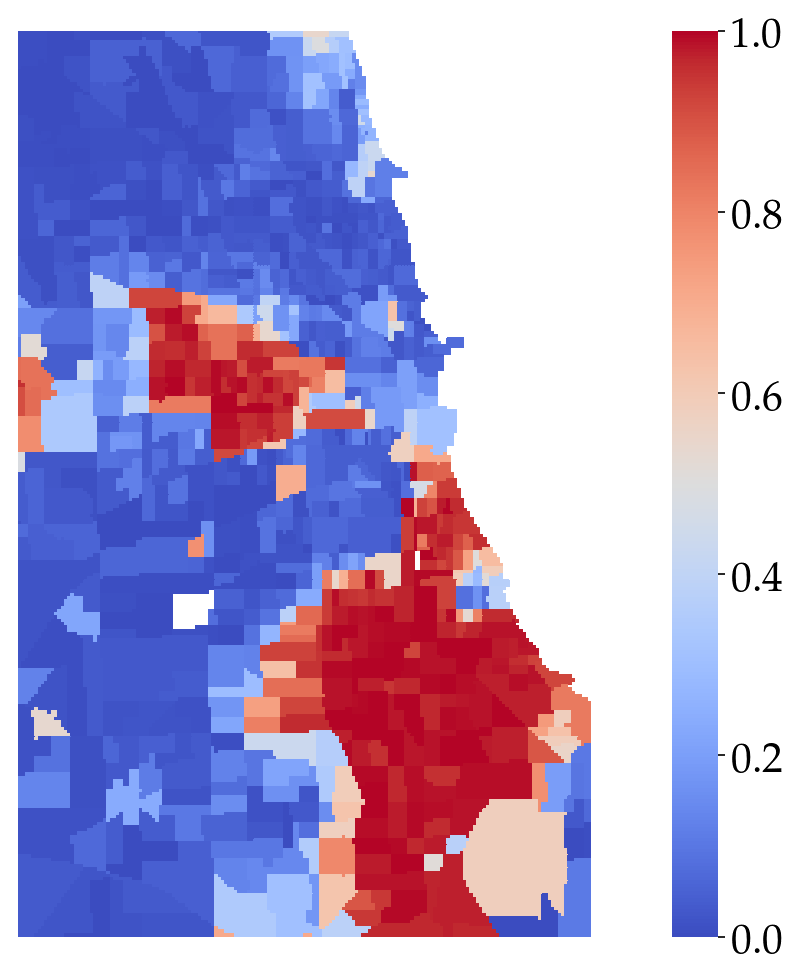
\includegraphics[height=.4\textheight]{gfx/HeatmapBlack.png}} \quad
    \subfloat[Average \pp predicted values $f$ in the year 2015]
    {\label{fig:heatmap_predicted}%
        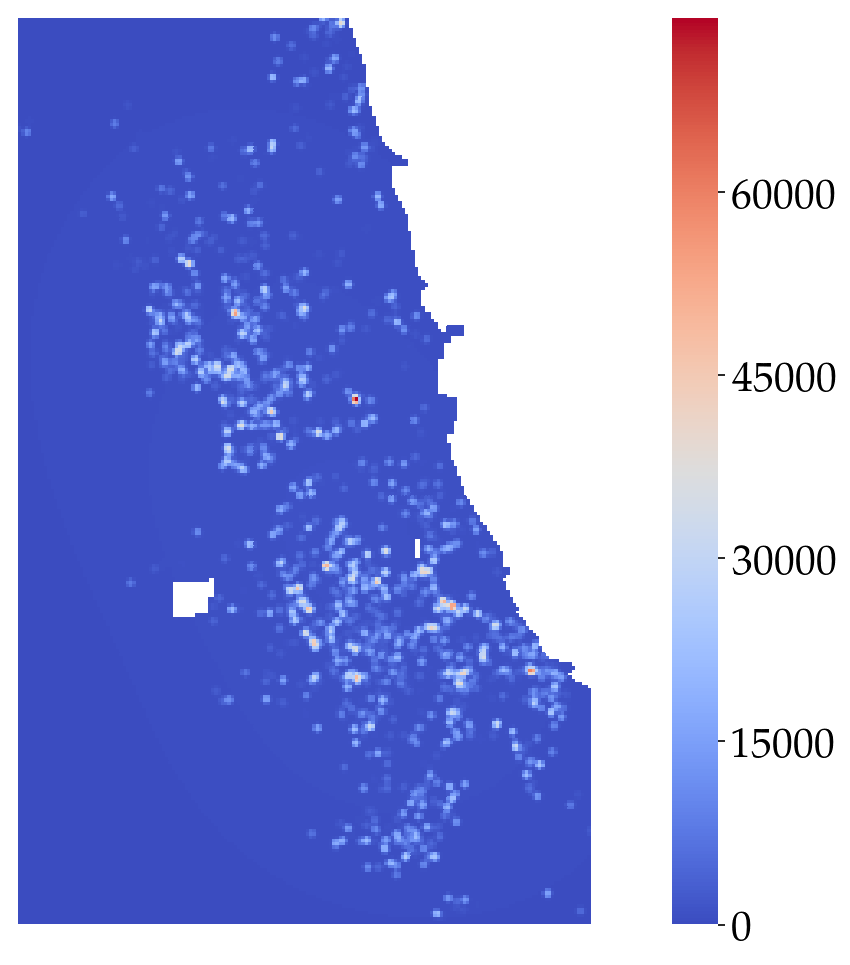
\includegraphics[height=.4\textheight]{gfx/HeatmapPredicted.png}} \\
    \caption{The visual correlation between race and \pp}
    \label{fig:heatmaps_correlation}
\end{figure}
Fairness through unawareness reflects a variety of intuitive beliefs about fairness. One intuition suggests that fairness through unawareness is the best that decision-makers or classifiers can hope for, because any other correlation between a protected attribute and the predictions might be explained as an unfortunate reflection of real-world correlation between the protected attribute and the target variable of prediction (in this case, criminality of a location). From this viewpoint, the results of \pp ought to be taken as is without modification. Other definitions of fairness attempt to take the problem of proxy discrimination seriously and control for it.

\section{Three Common Definitions}

Using conditional independence, three common definitions of fairness can be stated compactly as relationships between the ground truth $Y$, the prediction $\hat{Y}$, and the protected attribute $A$.\footnote{As a reminder of notation, the statement, "Random variable $X$ is independent of random variable $Y$ given the observation of random variable $Z$" is written as $X \perp Y \mid Z$.} Each of these definitions is observational in the sense that one does not need to conduct an intervention or run an experiment to order to assess them (causal notions of fairness do require interventions) \citep{hardt_equality_2016}. One of these definitions attempts to allow for the sort of proxy discrimination exhibited in this example up to the extent that is justified by correlation between the protected attribute and the true status. This definition also turns out to be relatively strong, insofar as it sometimes requires the decision-maker to make sacrifices to accuracy and even other notions of fairness.

The first definition, demographic parity ($\hat{Y} \perp A$), strengthens the "fairness through unawareness" condition, but ultimately to an unrealistic degree. Not only do the predictions have to be made without the protected attribute, the final predictions must also be statistically independent from the predicted attribute. This is a very stringent fairness requirement, since, as we have already seen, $Y$ and $A$ are related, and $\hat{Y}$ wants to track $Y$. Demographic parity further formalizes the notion of fairness that fairness through unawareness attempts to satisfy: in the ideal world, the true variables $Y$ are independent from protected attributes $A$. Thus, in the ideal world, either fairness through unawareness or demographic parity are sufficiently strong notions of fairness.

The next definition, equalized odds ($\hat{Y} \perp A$ | Y), can be seen as a relaxation of the previous criterion. After conditioning on the true status, the predictions ought to be independent from group status. This definition of fairness formalizes the amount of correlation that is permissible between the prediction $\hat{Y}$ and the protected group $A$: exactly as much as would be useful to predict true status.

Unlike the next and final fairness definition, which attempts to equalize accuracy across protected groups, equalized odds attempts to equalize false positive and negative rates across protected groups. The normative implications of this difference are significant, since false positives and negatives can have differing consequences on the individual and the community \citep{narayanan_21_2018}. In policing, a false positive might introduce an innocent individual into the criminal justice system, while a false negative might leave a criminal at large. In predictive policing, the individual units who are subjected to policing might be considered individual persons or the neighborhoods and locations which are recommended for patrol. If the individual units are locations, then the implication of a false positive is overpolicing a community unjustly while the implication of a false negative is underpolicing a community unduly. Equalized odds is a fairly stringent notion of fairness because satisfying it often requires sacrifices to accuracy \citep{hardt_equality_2016}.

Finally, sufficiency ($Y \perp A \mid \hat{Y}$) requires that the algorithm's overall accuracy across different groups is the same. Put differently, the location of the grid cell ought to be sufficient information for prediction and further conditioning on race (in addition to the prediction $\hat{Y}$) would not add any accuracy. This is the least stringent fairness requirement, and many out-of-the-box ML algorithms already satisfy this criterion \citep{barocas_fairness_2018}. One might intuit sufficiency in the context of predictive policing as follows: if one race is responsible for $p\%$ of the overall crime, then that race ought to be policed $p\%$ of the time.\footnote{Out of the box, \pp does not appear to satisfy this definition of fairness (\autoref{sec:sufficiency}). The upshot is that the predicted intensities from \pp have different interpretations based on the demographic makeup of the grid cell, a line of inquiry which is not pursued in this research.}

Sufficiency and equalized odds are incompatible whenever the baseline rate of true status differs between groups \citep{kleinberg_inherent_2016,chouldechova_fair_2017}.\footnote{\autoref{proof:ch_3} offers an alternative proof of this incompatibility using the $p\%$ intuition for sufficiency suggested above.} In the real-world, one can usually only ask that either sufficiency or equalized odds are met.

We will assess \pp on and make \pp fairer with respect to equalized odds because equalized odds is a stronger notion of fairness than sufficiency without being obviously deficient like demographic parity. Sufficiency is too weak a notion of fairness because it ignores the consequential difference between false positives and negatives in many contexts. Some have argued that because of the impossibility of achieving both equalized odds and sufficiency, one ought to focus on deploying predictors which are as accurate as possible while also ensuring that the processes around the predictor are also just \citep{corbett-davies_algorithmic_2017}. Essentially, this view bites the bullet on the impossibility theorem, and accepts the fact that equalized odds will not be met in real-world scenarios. While there is some merit to this view, especially since observational notions of fairness themselves do not guarantee that algorithms are used justly, there are likely still scenarios in which having an equalized odds predictor would be useful. Moreover, the aim of this thesis is to show how \pp fails to impress either on accuracy or on a relatively stringent notion of fairness. We do not claim to have the final word on all normative concerns surrounding algorithmic fairness.
% Since \pp by default satisfies sufficiency, equalized odds will be the target metric of fairness for the present research. However, that does not discount the viewpoint of sufficiency (or fairness through unawareness). This paper takes both the perspective of no fairness constraints---accuracy is the only important criterion---and of relatively strong fairness constraints. We will show how \pp, scored on either accuracy or equality of opportunity, fails to impress.

Finally, as a cautionary note regarding the usage of technical notions of fairness, ensuring equalized odds in predictions does not guarantee the equal distribution of risk or burden in reality. For example, in the context of predictive policing, individuals may still face heightened scrutiny for their racial features, regardless of which grid cells \pp ultimately predicts. The task of equalizing burden in practice requires, as \citet{perry_predictive_2013} suggested, best practices throughout the whole policing pipeline.

%************************************************
\chapter{\pp with Equalized Odds}\label{ch:fairpol}
%************************************************

In the previous chapter, we described various notions of fairness and settled upon equalized odds as the object of measurement for this study. In this chapter, we now focus on the computational task of ensuring equalized odds in \pp (and theoretically, any predictive policing algorithm). The main theoretical contribution of this chapter is a post-processing task for approaching equalized odds. The task "post-processes" the predicted values of \pp and does not modify the internal model of \pp. Any predictive policing algorithm which also meets the description of the predictive policing task in \autoref{ch:predpol_primer} can also be modified using the following work.

The intuition for the post-processing modification is that if equalized odds is true, then the following quantity should be close to zero:
\begin{align}
    \left|\text{\% black crime caught} - \text{\% white crime caught}\right| \label{eq:unfairness_measure}
\end{align}
This measure captures the belief that grid cells with equal amounts of criminal activity ought to have similar predicted intensities, regardless of their demographic make-up. This measure also solves the problem that while observational notions of fairness are frequently deployed on binary variables, the variables in our setting (the predicted intensity per grid cell, the demographic make-up per grid cell, and the number of crimes in each grid cell) are all continuous.

\autoref{eq:unfairness_measure} is properly a measure of \emph{un}-fairness, since smaller values of it correspond to fairer predictions and vice versa. One can turn \autoref{eq:unfairness_measure} into a fairness measure by subtracting it from $1.0$.

The vague terms "black crime" and "white crime" accommodate both different interpretations of what fairness in policing requires and the possibilities afforded by different datasets. For example, the Chicago crime data used for the present research omits race as a feature of each observation. Instead, we operationalize "black crime" and "white crime" as "crime occurring in locations with larger black or white populations" respectively.\footnote{To do so, we combined the Chicago crime data with other demographic data; see \autoref{app:methodology} for details.} In other scenarios, researchers may choose to prioritize the race of either the perpetrator of a crime or the race of the victims; the approach used in this research attempts to consider both.

Given the goal of catching equal amounts of crime across protected groups, one ought to try and equalize the predicted intensity of crime across protected groups in the locations visited. To formalize this notion for the $i$th grid cell, let $f_i$ be the intensity, as predicted by PredPol, $b_i$ the percentage of black individuals, and $w_i$ the percentage of white individuals. The data are processed so that $\forall i$, $b_i + w_i = 1.0$. First, compute:
\begin{align}
\hat{f}^{\text{(black)}}_i &= \frac{b_i f_i}{\sum_i b_i f_i} \label{eq:f_hat1}\\
\hat{f}^{\text{(white)}}_i &= \frac{w_i f_i}{\sum_i w_i f_i} \label{eq:f_hat2}
\end{align}
The $\hat{f}$ values indicate \emph{racially-differentiated predictive
value}.\footnote{If one had race information available for the perpetrator (or victim) of each crime, they could separately estimate intensities for each race $f^{\text{(black)}}, f^{\text{(white)}}$, and combine them in the following way: $
\hat{f}^{\text{(black)}}_i = \frac{f^{\text{(black)}}_i}{\sum_i f^{\text{(black)}}_i}$ and $
\hat{f}^{\text{(white)}}_i = \frac{f^{\text{(white)}}_i}{\sum_i f^{\text{(white)}}_i}
$} If one is concerned about crime that disproportionately affects black communities, they should visit grid cells as ranked by the value of $\hat{f}^{\text{(black)}}_i$, and vice versa for white communities. In a world where communities are fully integrated and there are no global disparities in demographics (so the demographics of each grid cell reflect the demographics over all locations), $\hat{f}^{\text{(black)}}_i = \hat{f}^{\text{(white)}}_i$ for all $i$. In this ideal setting, one could also achieve demographic parity.

Now, we can calculate the \emph{predictive value gap} for each grid cell $i$ by taking $\Delta_i = |\hat{f}^{\text{(black)}}_i - \hat{f}^{\text{(white)}}_i|$.
% The values in figures~\ref{fig:fair_overall} and \ref{fig:fair_detail} are computed in this way.
Note that the values of $\hat{f}$ are in the unit interval $[0, 1]$.
Thus, the difference $\hat{f}^{\text{(black)}}_i - \hat{f}^{\text{(white)}}_i$ will be in the range $[-1, 1]$, and $\Delta_i$ will be in the unit interval as well. When $\Delta_i = 0$ for a particular grid cell, it means that that grid cell captures an equal amount of crime affecting both races; in other words, that grid cell is "fair."

With the definitions of $\hat{f}$ in hand, we can define the post-processing fairness task, which takes its inspiration from the knapsack problem in theoretical computer science. Intuitively, even if no grid cell is fair individually, different combinations or subsets of grid cells might be fair (as indicated by their summed differences $\hat{f}^{\text{(black)}}_i - \hat{f}^{\text{(white)}}_i$.\footnote{We must drop the absolute value around this expression in order to allow different gaps from different cells to cancel out.} This problem mirrors a knapsack task: we want to maximize the overall value of a subset of items from a larger collection while subject to certain constraints.

More formally, given a list of $N$ items, each with an associated benefit $f_i$ and two different costs $\hat{f}^{\text{(black)}}_i$ and
$\hat{f}^{\text{(white)}}_i$, find a subset of at most $k$ items such
that: the total benefit is maximized, and the two total costs are approximately equivalent. If we let $x_i$ be a binary indicator for whether an item is included in the knapsack, and give dummy weights of $w_i = 1$ for all $i$, we can state the problem as follows:
\begin{alignat}{2}
&\!\max_{x}        &\;& \sum_i f_i x_i\\
&\text{subject to} &  & \sum_i x_i = k\\
&                  &  & \sum_i
\hat{f}^{\text{(black)}}_i x_i = \sum \hat{f}^{\text{(white)}}_i
x_i
\intertext{The tricky condition is the third line, which we can transform into two constraints:}
&\!\max_{x}        &\;& \sum_i f_i x_i\\
&\text{subject to} &  & \sum_i x_i = k\\
&                  &  & \sum_i \hat{f}^{\text{(black)}}_i x_i = D\\
&                  &  & \sum_i \hat{f}^{\text{(white)}}_i x_i = D
\end{alignat}
The value $D$ is arbitrary---if the subset of grid cells selected polices the same percentage of black and white crime, then the subset is fair, by our standard. However, when implementing this problem in practice, we also relax all of the equalities to be less-thans. Then, $D$ takes on the role of the \emph{maximum tolerable gap} in fairness. Because the constraints become inequalities, the gap in fairness will be at most $D$.

We also observe that without the fairness constraints (alternatively, setting $D = 1$), this knapsack problem is trivial and amounts to taking the $k$ cells with highest $f_i$ value.

To provide further intuition for how this post-processing task might affect the predictions of an unconstrained procedure, we will consider two toy examples that illustrate the two possible ways in which post-processing task changes predictions. Each example considers a map of crime with four grid cells, and the resource-strapped police department can only visit two of the locations. Each map is represented by a two-by-two table, where the contents of each cell respectively indicate the predicted crime intensity $f$, the amount of black crime (as a percentage of all black crime) occurring in that cell $f^{\text{(black)}}$, and the same quantity for whites $f^{\text{(white)}}$. We further assume that we have a perfect predictor, so that $f = \hat{f}$.

\begin{table}[h]
\centering
\resizebox{0.5\textwidth}{!}{%
\begin{tabular}{|l|l|}
\hline
5 / 0.4 / 0.2 & 4 / 0.2 / 0.2 \\ \hline
4 / 0.2 / 0.2 & 1 / 0.2 / 0.4 \\ \hline
\end{tabular}%
}
\caption{Example 1: A four-cell world}
\label{table:example1}
\end{table}

In example 1, the unconstrained algorithm would visit the top-left cell and either the cell to the immediate bottom or right to capture:
\begin{itemize}
    \item 9 units of crime
    \item 60\% of black crime
    \item 40\% of white crime
\end{itemize}
However, the post-processing fairness modification with a sufficiently low tolerance threshold ($D < 0.2$) would choose both the top-right and bottom-left cell instead and thus capture:
\begin{itemize}
    \item 8 units of crime
    \item 40\% of black crime
    \item 40\% of white crime
\end{itemize}
This example illustrates that the fair procedure will generally prefer cells which have smaller $\Delta_i$ values. Moreover, the accuracy of the fair procedure will degrade further as the "unfair" cells account for more of the overall crime (for example, let the 5 in the top-right cell be 50 or 500).

The fair procedure would also prefer combinations of cell that have a collectively small $\Delta_i$ value, as the second example will illustrate:
\begin{table}[ht]
\centering
\resizebox{0.5\textwidth}{!}{%
\begin{tabular}{|l|l|}
\hline
5 / 0.4 / 0.2 & 4 / 0.2 / 0.2 \\ \hline
1 / 0.2 / 0.2 & 3 / 0.2 / 0.4 \\ \hline
\end{tabular}%
}
\caption{Example 2: Another four-cell world}
\label{table:example2}
\end{table}

The unconstrained algorithm would choose the top row of cells and, as before, capture:
\begin{itemize}
    \item 9 units of crime
    \item 60\% of black crime
    \item 40\% of white crime
\end{itemize}
The post-processing fairness modification with a sufficiently low tolerance threshold ($D < 0.2$) would instead choose the top-left and bottom-right cell and capture:
\begin{itemize}
    \item 8 units of crime
    \item 40\% of black crime
    \item 40\% of white crime
\end{itemize}
In this situation, the fair procedure achieves greater fairness by "balancing" the unfairness of one cell with the unfairness of another cell. In this situation, the accuracy of the fair procedure degrades based on the difference between the second-best cell (the top-right cell in this example) and the "balancing" cell.

%************************************************
\chapter{Results}\label{ch:results}
%************************************************

In this chapter, we present the major results from simulated tests on the Chicago crime data set. First, we find that the accuracy of \pp does not exceed a baseline heuristic in the top 5\% of cells predicted. Second, we find that \pp, as assessed by the measure discussed in the previous chapter, is not fairer than the baseline heuristic. Third, we find that the fairness modifications presented in the previous chapter can work decently well at improving fairness while preserving the accuracy of \pp. Taken together, these results show that the benefits of \pp are overstated. We discuss this possibility as well as other implications in the next chapter.

\section{Accuracy}
\autoref{fig:accuracy} shows the accuracy of \pp compared to completely random prediction and the baseline measure, "naive counting." The baseline measure is comparable to a naive Bayes approach to predictive policing: rank each grid cell by the number of crimes that have taken place in that location over the whole observed dataset. In the language of \citet{mohler_marked_2014}, the naive counting measure corresponds to the "chronic hotspots" method with no decay in time (observations further back in time are weighted equally as more recent ones).
\begin{figure}[bth]
    \myfloatalign
    \subfloat[Overall, \pp predicts well...]
    {\label{fig:accuracy_overall}%
        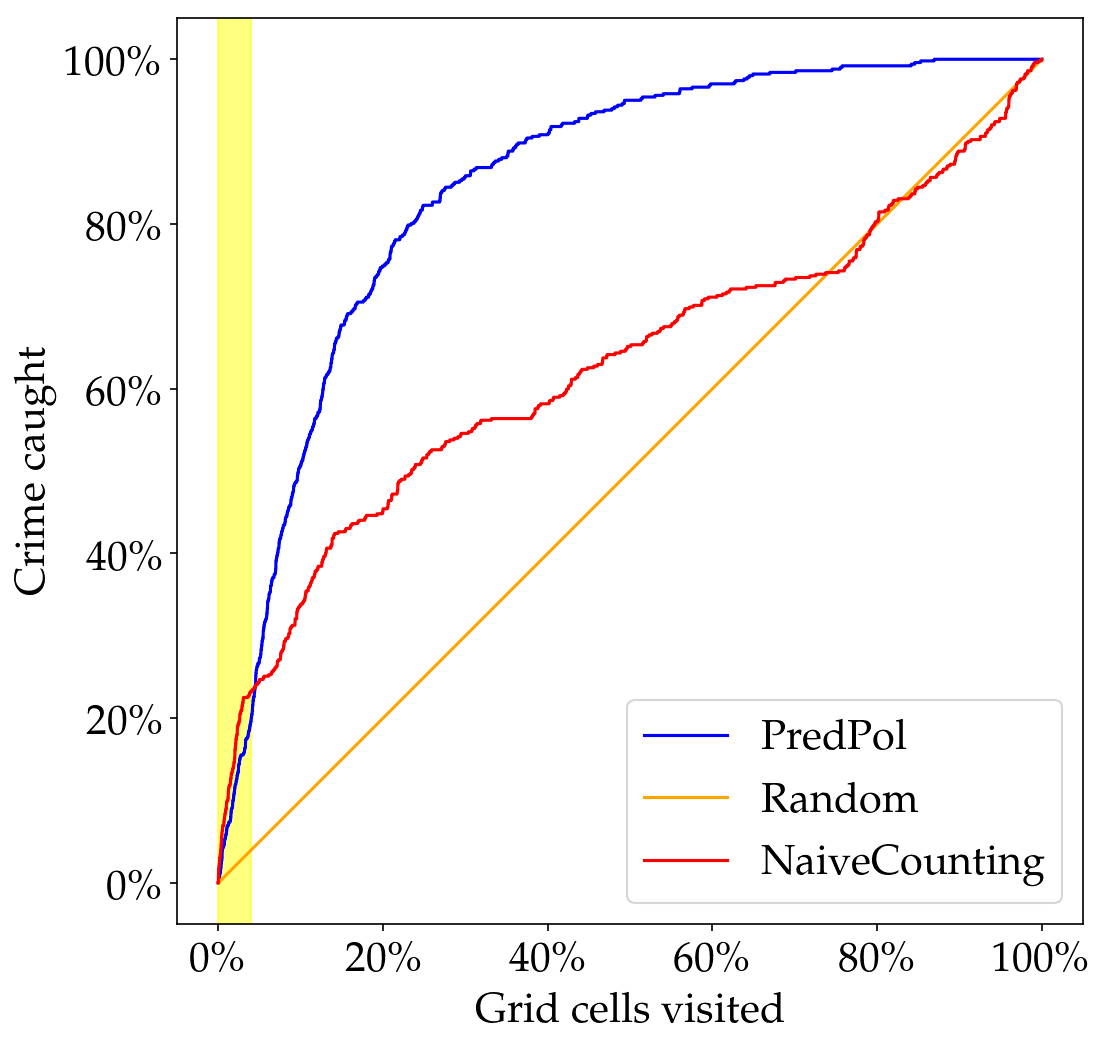
\includegraphics[width=.36\linewidth]{gfx/AccuracyAll.png}} \quad
    \subfloat[...but not in the top 5\% of grid cells.]
    {\label{fig:accuracy_zoom}%
        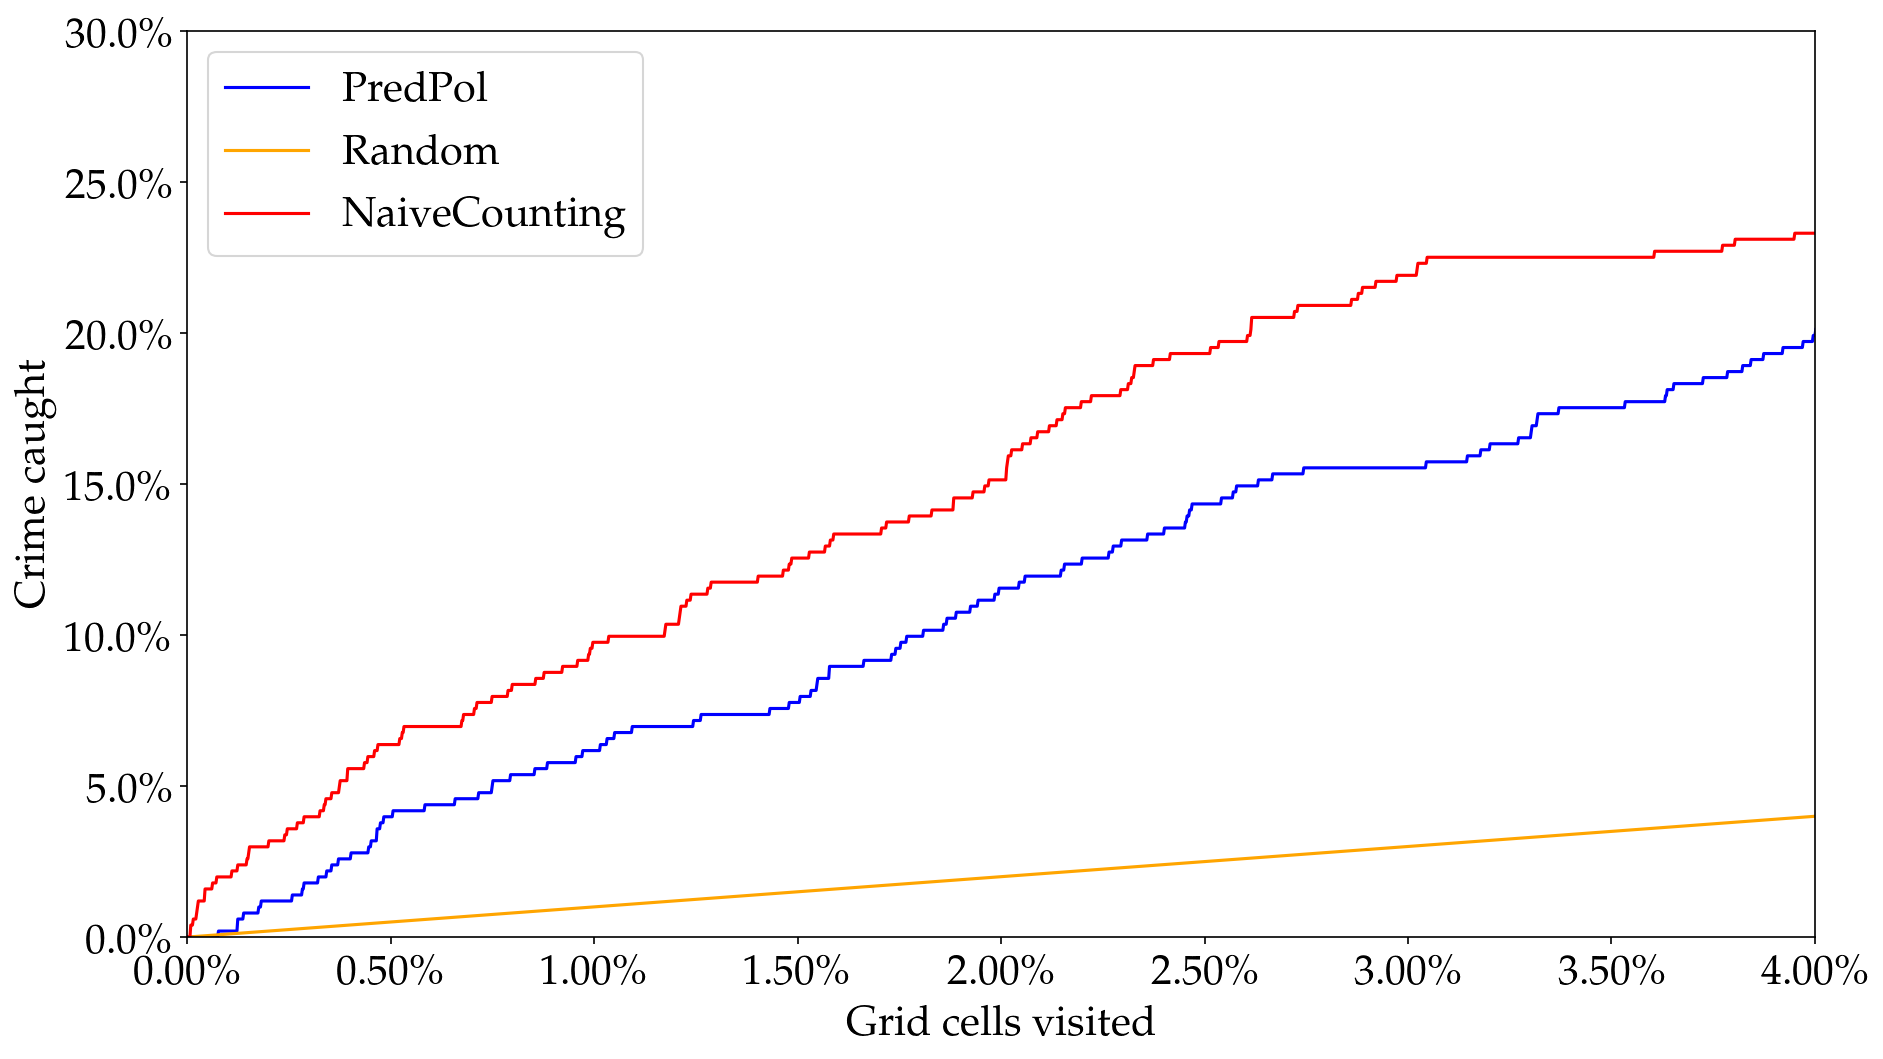
\includegraphics[width=.6\textwidth]{gfx/AccuracyZoom.png}} \\
    \caption[Accuracy curves comparing \pp and other baselines]{Accuracy curves comparing \pp and other baselines}\label{fig:accuracy}
\end{figure}
The results are shown as a function of the number of grid cells visited, since visiting more grid cells will tend to improve accuracy in general (these curves are similar to ROC curves in binary classification). The y-axis plots the percentage of crime caught, or the number of crimes that occur in the cells predicted as a percentage of the total crime occuring that day. Each curve is an average over 365 days of prediction in 2015.

Imagining that one had access to a perfect oracle, which knew in advance where each crime would occur, the results from such an oracle would plot a nearly perfect right angle at the upper left of \autoref{fig:accuracy_overall}. This reflects the fact that tiny percentage of grid cells each day are responsible for crime; knowing those locations in advance means that all of the crime occurring in a day could be captured by visiting just a few locations.

\pp shows increased accuracy when considered over the whole range of grid cells. The naive counting measure breaks down at around 80\% of grid cells predicted, when its performance becomes no better than randomly guessing.

However, visiting even 10\% of the grid cells on a map is unreasonable for police departments to accomplish. \citet{mohler_marked_2014} states that "a range of 250–500 150m $\times$ 150m cells is a realistic number for a city the size of Chicago," which correspond on the above plots to a range of $0.5\%$ to $1\%$ of grid cells.

\section{Fairness}
\autoref{fig:fairness} assesses the fairness of the same measures discussed in the previous section. Again, the x-axis is the percentage of grid cells visited/used by the algorithm. The y-axis computes the percentage of black crime captured (by the x\% grid cells predicted by the algorithm) minus the percentage of white crime captured (by the x\% grid cells predicted by the algorithm). When all grid cells have been predicted, 100\% of crime of both races has been captured, so each of the curves in figure~\ref{fig:fairness_overall} meet at $(1.0, 0.0)$.

A completely fair algorithm, by this metric, would lie directly on the x-axis. Random prediction has this property (noise in the curve is due to the random variation, and on different runs, the shape of the curve changes completely). It is interesting to note that random prediction is fair with regard to equalized odds while at the same time qualifying as a "fair through unawareness" classifier. Of course, the accuracy of predicting randomly leaves much to be desired. Perfect prediction also lies on the x-axis, since perfect prediction captures all crime nearly instantaneously, thus also capturing equal percentages of both races' crimes. Curves above the x-axis indicate some amount of bias against blacks, while curves below the x-axis indicate some amount of bias against whites. However, because of how we operationalized race and fairness in \autoref{ch:fairpol}, one could easily draw the opposite conclusions: capturing a larger percentage of crime in black districts \emph{favors} blacks, and vice versa. We remain open to this alternative interpretation. The point is to try and achieve equality for both races.

\begin{figure}[bth]
    \myfloatalign
    \subfloat[\pp is slightly fairer over all cells...]
    {\label{fig:fairness_overall}%
        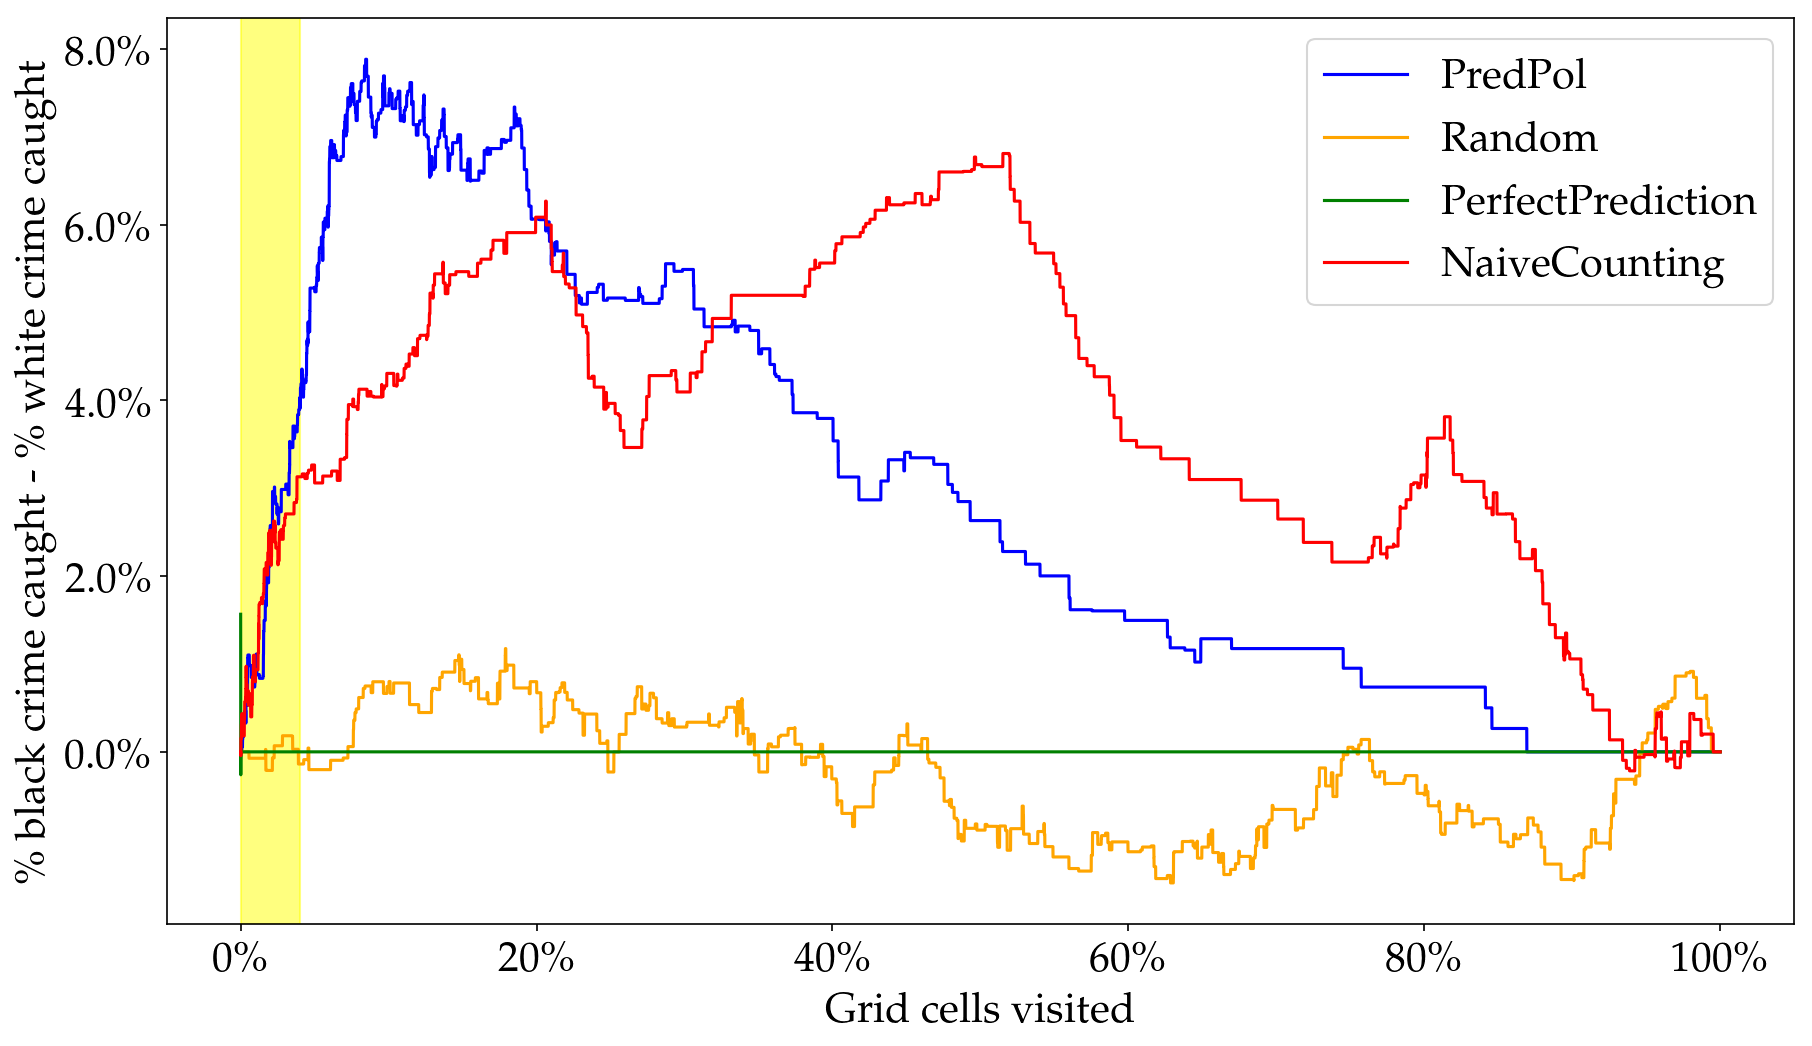
\includegraphics[width=.6\linewidth]{gfx/FairnessAll.png}} \\
    \subfloat[...but not especially so in the top 5\% of grid cells.]
    {\label{fig:fairness_zoom}%
        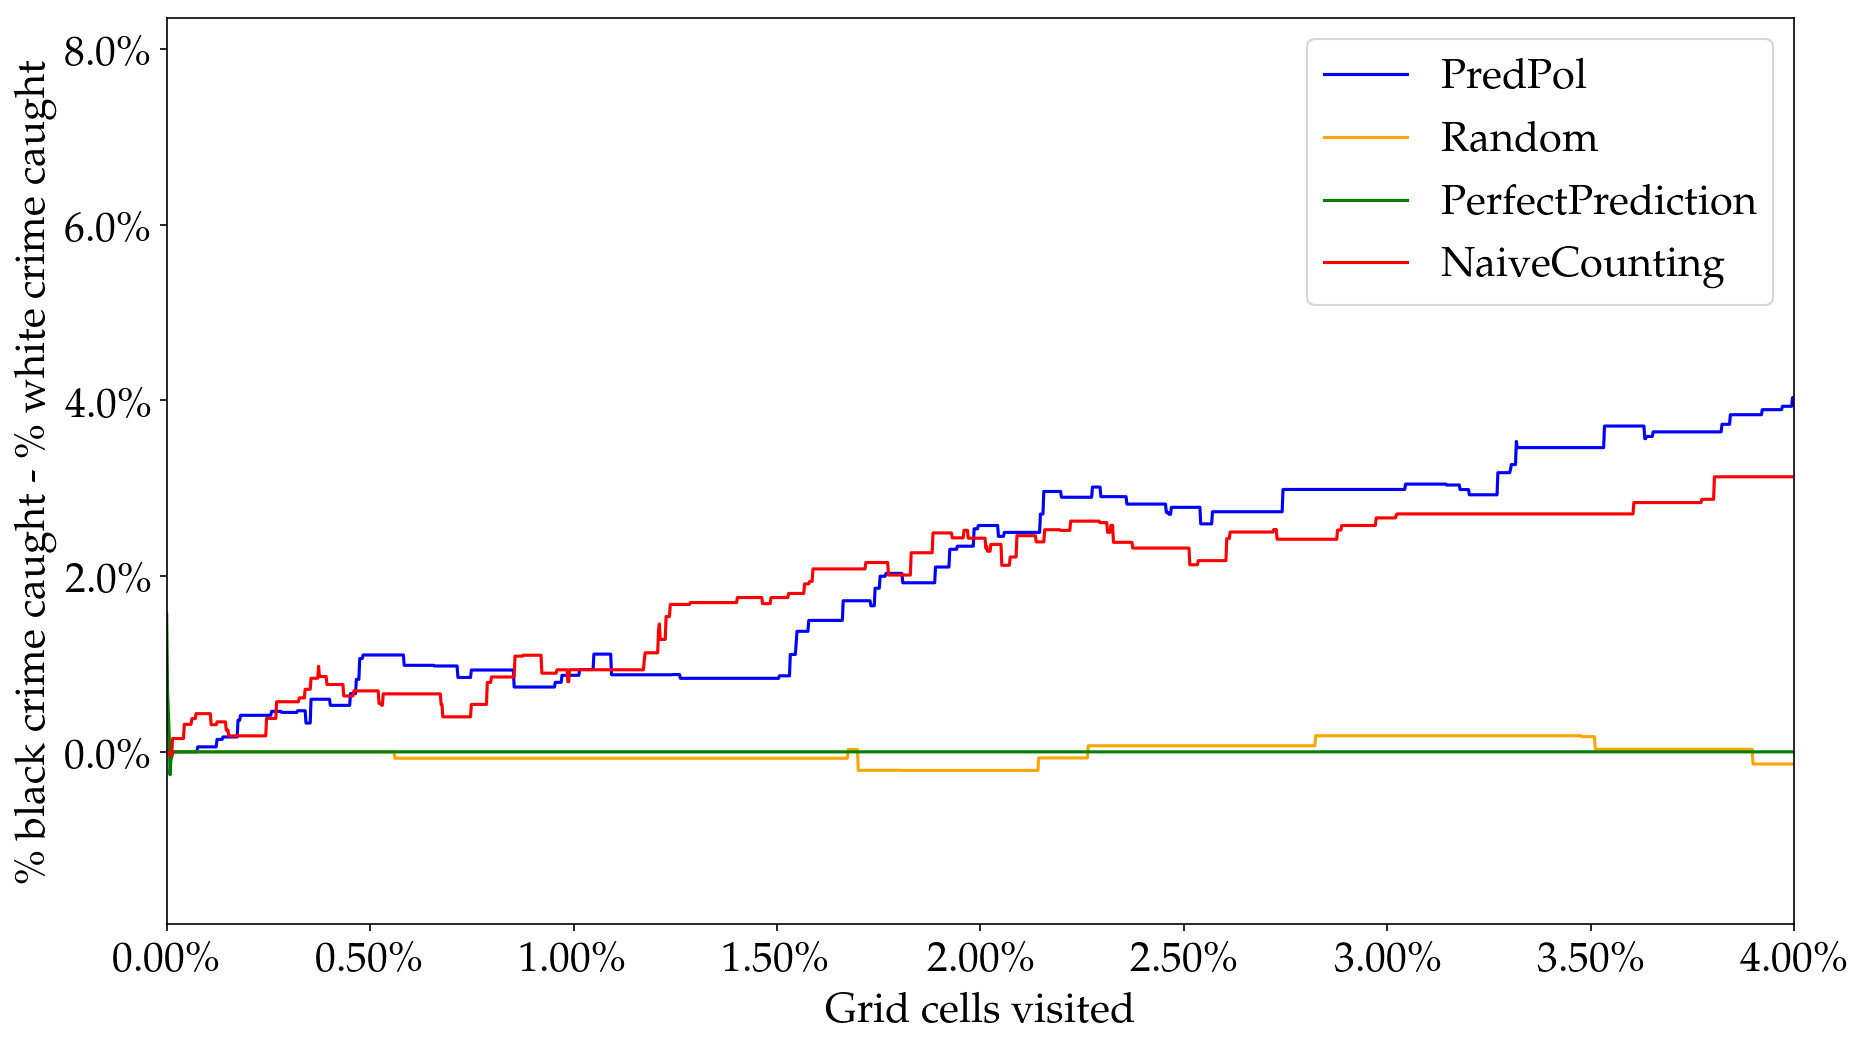
\includegraphics[width=.6\textwidth]{gfx/FairnessZoom.png}} \\
    \caption[Fairness curves comparing \pp and other baselines]{Fairness curves comparing \pp and other baselines}\label{fig:fairness}
\end{figure}

The differences between \pp and the baseline measure are less apparent on fairness. In the range of cells discussed in the previous section, \pp hews closer to the x-axis than the baseline measure.

One interesting aspect is that the fairness curves for both \pp and naive counting never go below the x-axis; in other words, both measures always capture a larger percentage of black crime than white crime. We suggest possible reasons for this in \autoref{sec:discussion}.

\section{Fairness Modification}
\begin{figure}[bth]
    \myfloatalign
    \subfloat[The modification has comparable accuracy...]
    {\label{fig:mkp_accuracy}%
        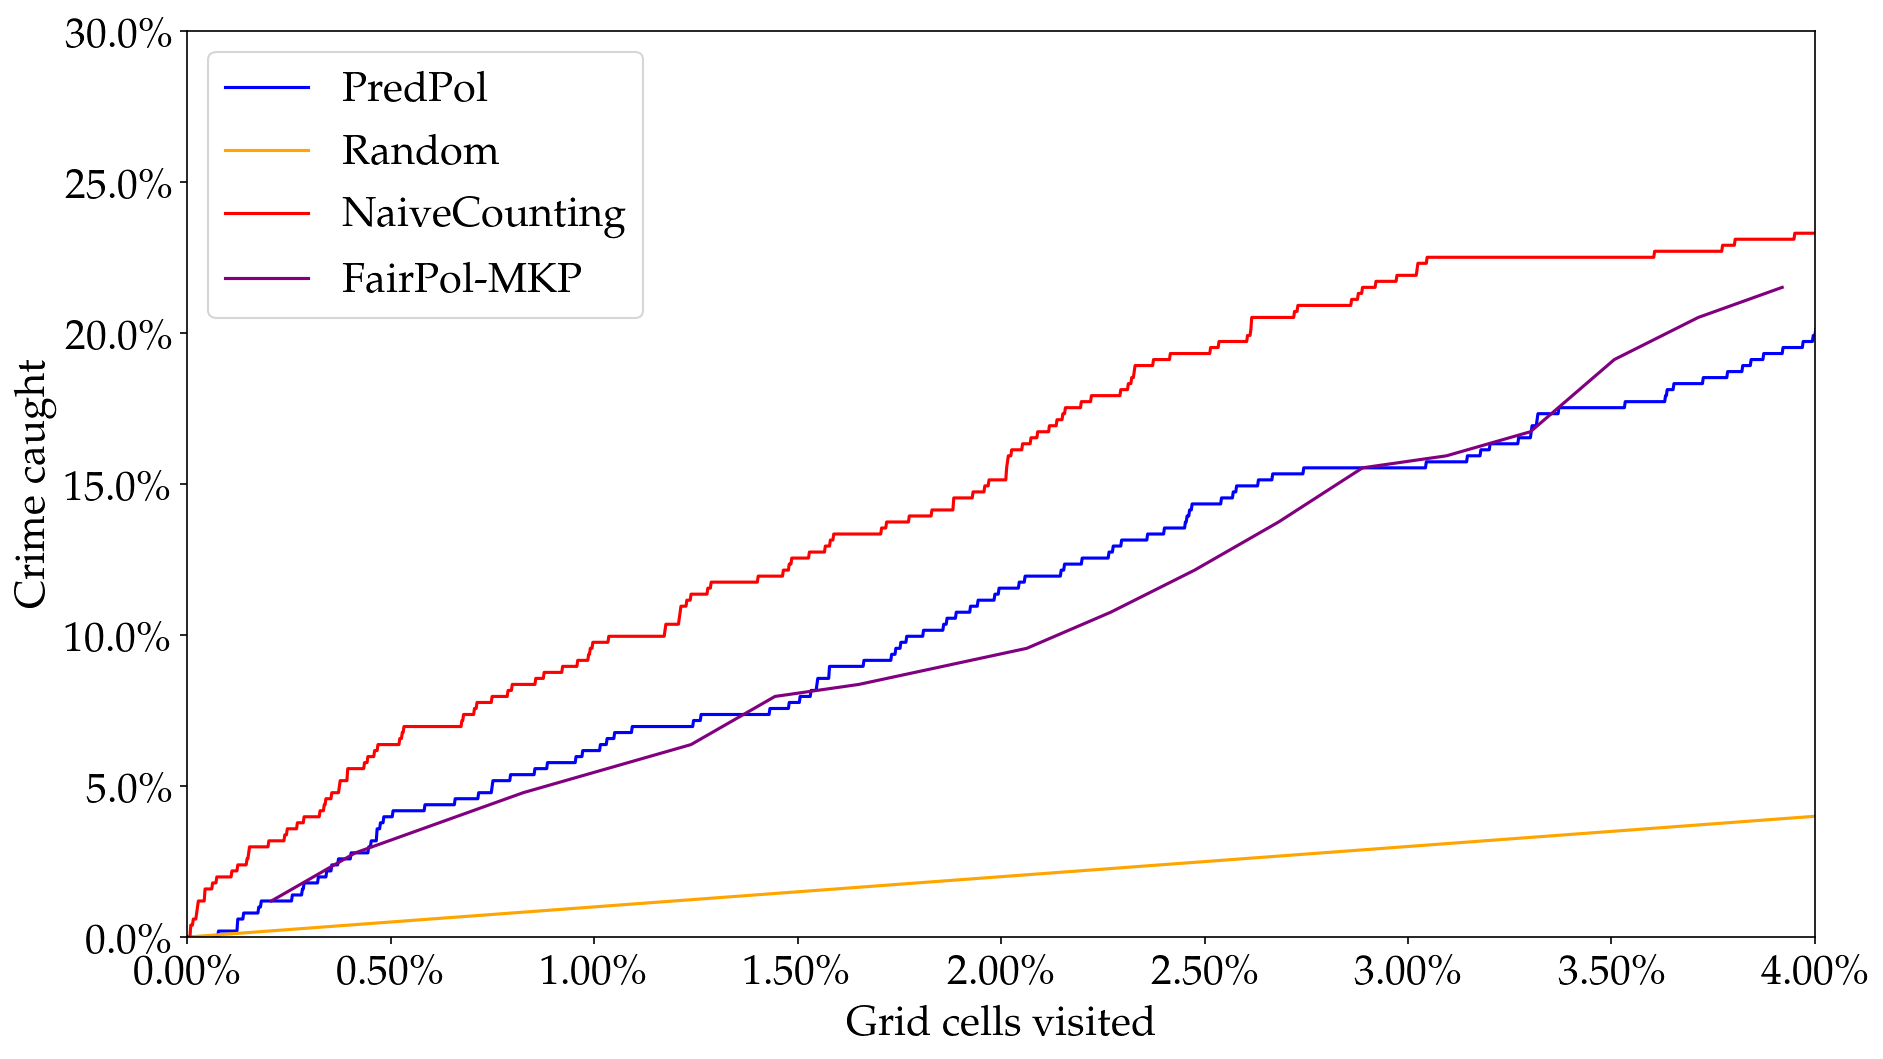
\includegraphics[width=.6\linewidth]{gfx/MKPAccuracy.png}} \\
    \subfloat[...while being significantly fairer.]
    {\label{fig:mkp_fairness}%
        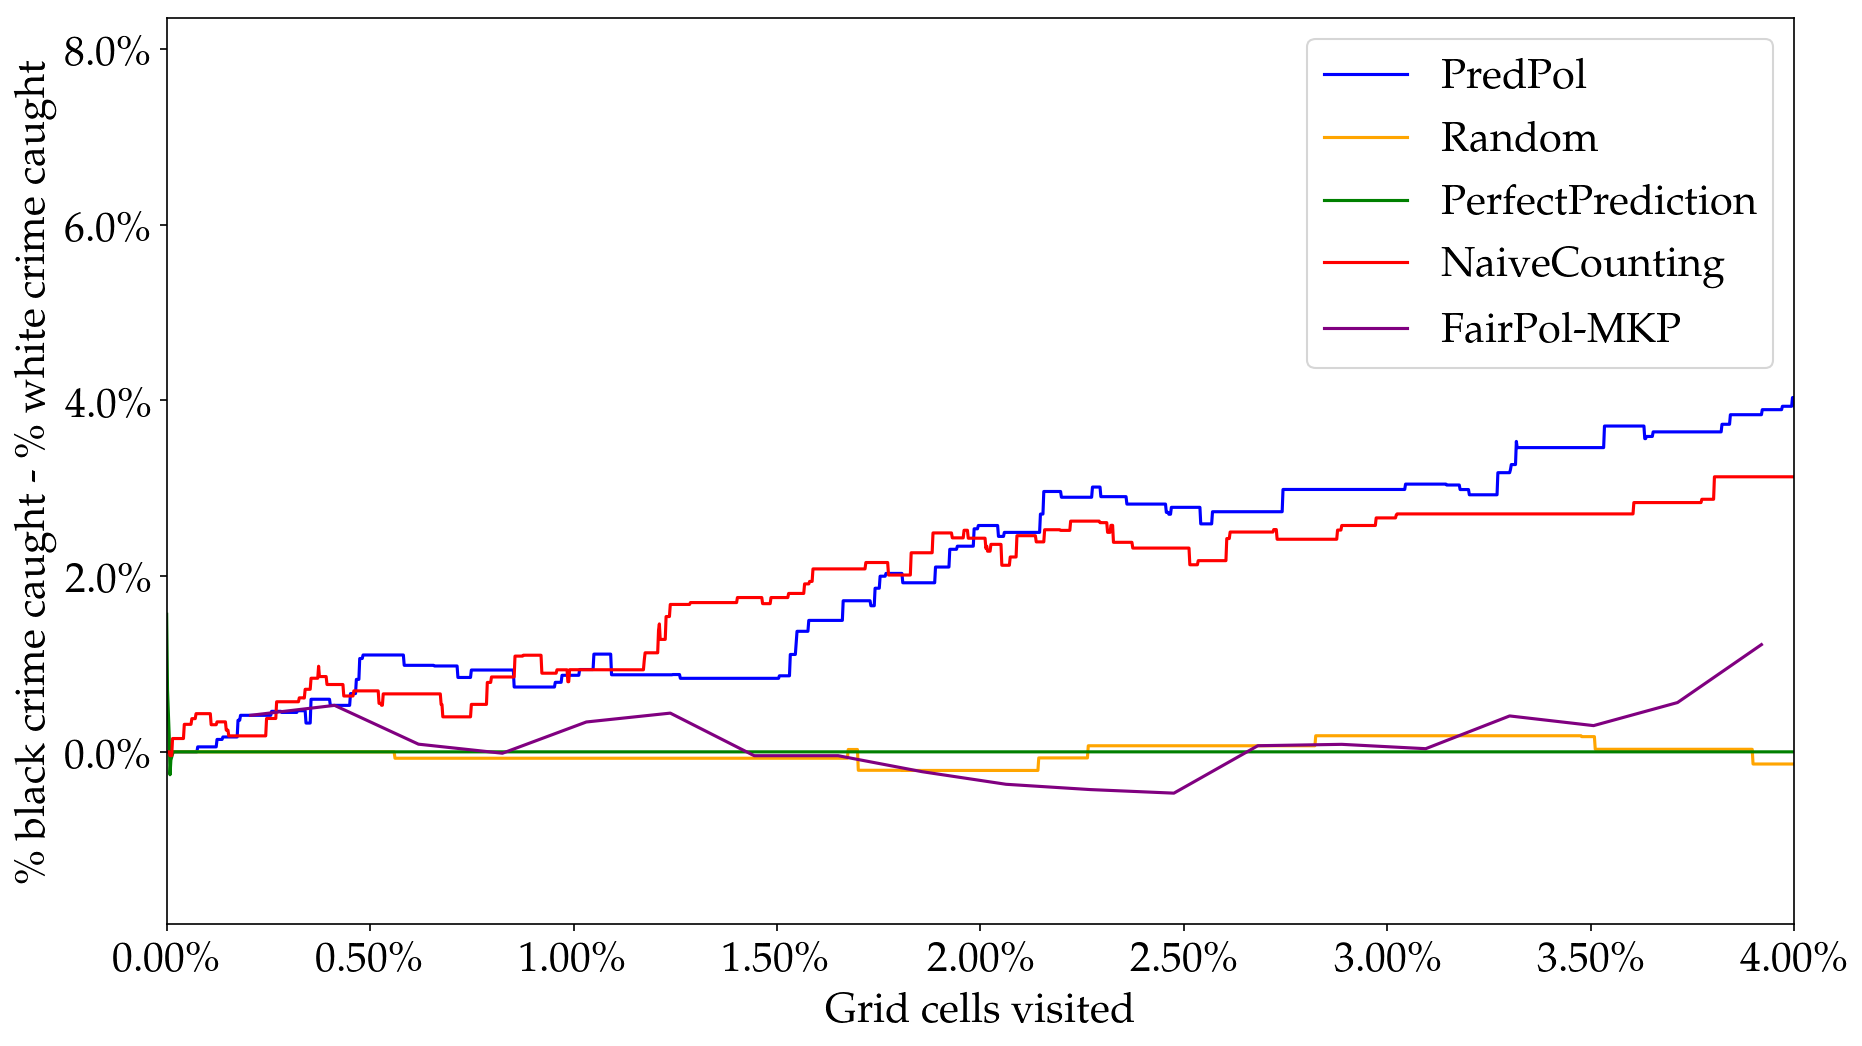
\includegraphics[width=.6\textwidth]{gfx/MKPFairness.png}} \\
    \caption[The accuracy and fairness of the post-processing modification]{The accuracy and fairness of the post-processing modification (purple) ($D = 1.25\%$)}\label{fig:mkp}
\end{figure}
Finally, \autoref{fig:mkp} shows the result of the post-processing task suggested in \autoref{ch:fairpol}. By seeking combinations of grid cells that together constitute fairer policing, these results show that achieving fairer prediction without comparable hits to accuracy is possible.

% TODO: Table: Numerical Summary of Results
% TODO: Translate the percentage differences into real-victimization (number of lives lost, affected)

\section{Caveats} \label{sec:caveats}

Before proceeding to a full discussion of the results we would like to, in the interest of transparency and future research, highlight several limitations of the present research. We omit using different types of crime to predict one another, as done in \citet{mohler_marked_2014}. That model uses the historical record of, say, burglaries, to assess increased likelihood of say, homicides. One direction for future research is to implement the full model described in \citet{mohler_marked_2014} and attempt to replicate the results of this research. Creating a plausible baseline method for this kind of prediction is complicated by the fact that different types of crime occur at very different rates than others; a naive Bayes method that treats all crime equally would be dominated by the most prevalent crime type.

Nevertheless, it still seems plausible that a baseline measure, such as the chronic hotspots method discussed in \citet{mohler_marked_2014} and similar to the naive counting measure used here, could achieve comparable performance to \pp. In several places throughout the text, \citet{mohler_marked_2014} also acknowledges that chronic hotspots account for most of the crime in the dataset. If this is indeed the case, then the discussion of ethics in the following section is still likely to hold merit. 

% Manual inspection of the figures in \citep{mohler_marked_2014} still suggest that the naive counting approach is comparable to the full marked point processes approach.

There are a few smaller differences that may have led to a difference in findings in the present research and \citet{mohler_marked_2014}. First, the number of grid cells in the simulation differs. It seems that Mohler examined a smaller geographical region than in the present research, but Mohler did not make note of this detail in their paper. Second, the Chicago dataset is known to change over time as the agency responsible for marinating the data re-randomizes the locations of crimes in order to protect privacy.

Finally, there may have been errors in our simulation, for which we take full responsibility. A more detailed explanation of methods along with replication code is available in \autoref{app:methodology}.

\section{Discussion} \label{sec:discussion}

Barring the caveats mentioned in the previous section, it is unclear why \pp does worse than the naive counting measure in the region specified. We hypothesize, for further testing, that some amount of constructive interference may be occurring: in the middle zone between two crime hotspots, \pp predicts a high amount of crime, despite being exactly in the middle of where the crime would likely occur.

With regard to normative issues, \citet{mohler_marked_2014} states that their model results in a 17\% relative improvement in accuracy from the measures they consider, and that, "[g]iven the high societal cost of homicide and serious gun crime (DeLisi et al., 2010), which is estimated to be billions of dollars a year in Chicago, even a few percent decrease in the homicide rate due to hotspot policing with a more accurate ranking method would be of significant societal benefit." Building off of the empirical results presented in this chapter, we posit that there may also be costs to fairness and transparency which should be weighed against the benefits of predictive policing. If a simpler method for prediction (i.e. the hotspot policing approach) is nearly as accurate, more equitable across protected groups, and easier to explain to the affected population, there are good reasons for preferring that simpler approach.
\begin{figure}[bth]
    \myfloatalign
    \subfloat[Black population as a percentage of total = black + white]
    {\label{fig:heatmap_black2}%
        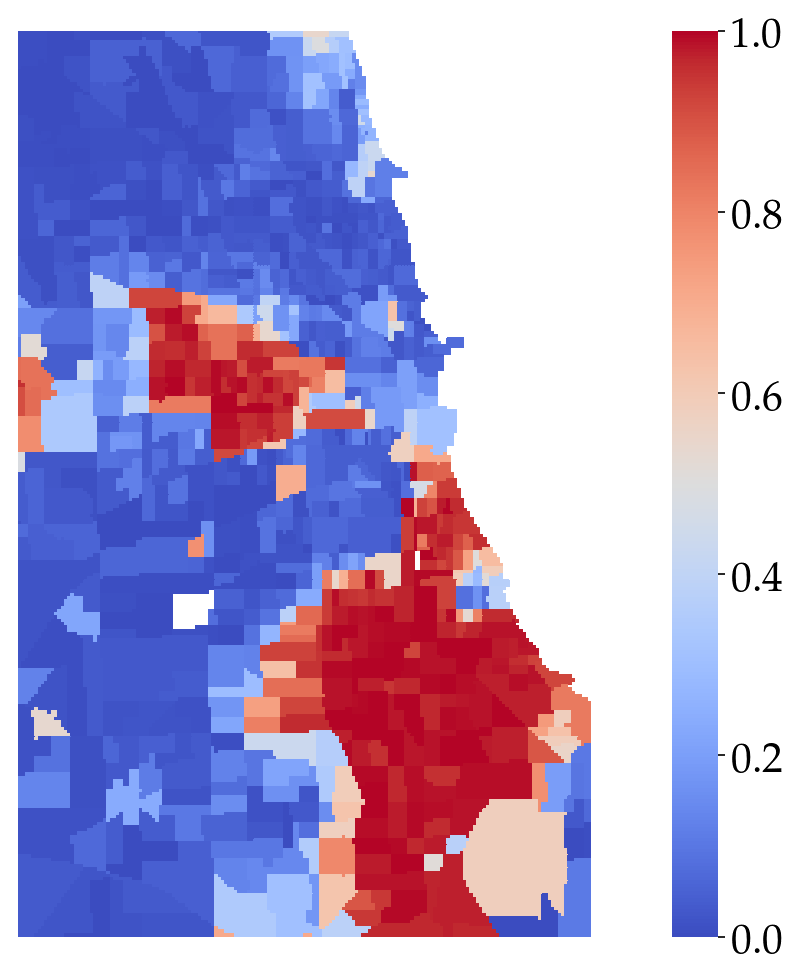
\includegraphics[height=.45\textheight]{gfx/HeatmapBlack.png}} \quad
    \subfloat[Number of actual crimes]
    {\label{fig:heatmap_actual}%
        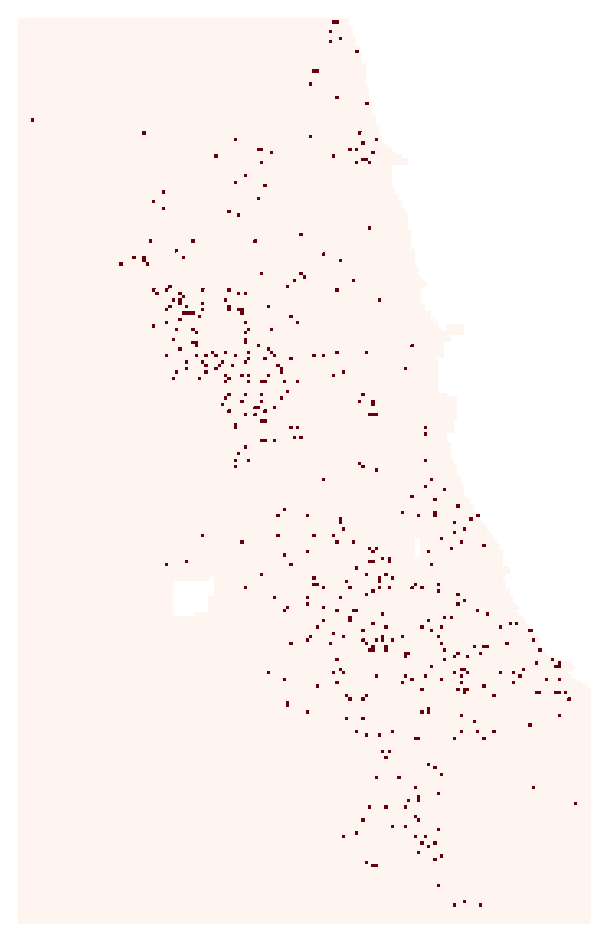
\includegraphics[height=.45\textheight]{gfx/HeatmapActual.png}} \\
    \caption{The visual relationship between race and actual number of crimes}
    \label{fig:actual}
\end{figure}

% Despite the success of machine learning in some areas, such as image recognition or playing games, algorithms in social applications have a much more difficult time achieving comparable success. The difficulty likely arises from the dearth of high-quality data and human understanding of the social phenomena that the algorithms interact with. Therefore, any purported accuracy benefits to a machine learning algorithm in a social application must be scrutinized carefully. It seems unlikely that we will see comparable improvements in accuracy in predictive policing as we have with, say, image or speech recognition.

Both \pp and naive counting police black crime more than white crime. We posit that this occurs because one group's crime is more concentrated in one area than another. \autoref{fig:heatmaps_f_hat} show the distribution of $\hat{f}$ values in the Chicago region while \autoref{fig:actual} shows the actual locations of crime. Since there is a weak relationship between race and number of crimes (as stated previously, Pearson's r of 0.11), we should expect crime in both whiter and blacker grid cells. However, the crimes in the whiter areas of the northern region are spread apart while the crime in blacker areas tends to be clustered closer together.

Because of \pp's aftershock model, it would tend to exploit the clustering of black crime and predict those regions more frequently, even though a good predictor would also try and account for the sparser crime occurring in the north of the map. That explains how \pp is initially more unfair than naive counting (in the range of 0-30\% cells predicted) in \autoref{fig:fairness_overall}. Nevertheless, \autoref{fig:fairness_zoom} does show that this difference in fairness is negligible in the range of grid cells that a police department could actually visit.

\begin{figure}[bth]
    \myfloatalign
    \subfloat[Where crimes affecting black...]
    {\label{fig:heatmap_pct_black}%
        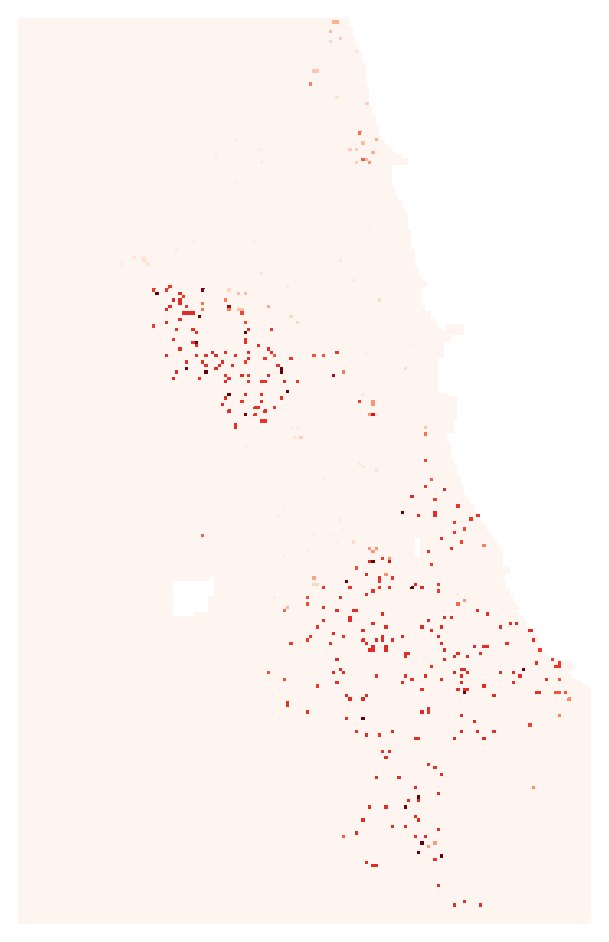
\includegraphics[width=.48\linewidth]{gfx/HeatmapPctBlackCrime.png}} \quad
    \subfloat[...and white people occur]
    {\label{fig:heatmap_pct_white}%
        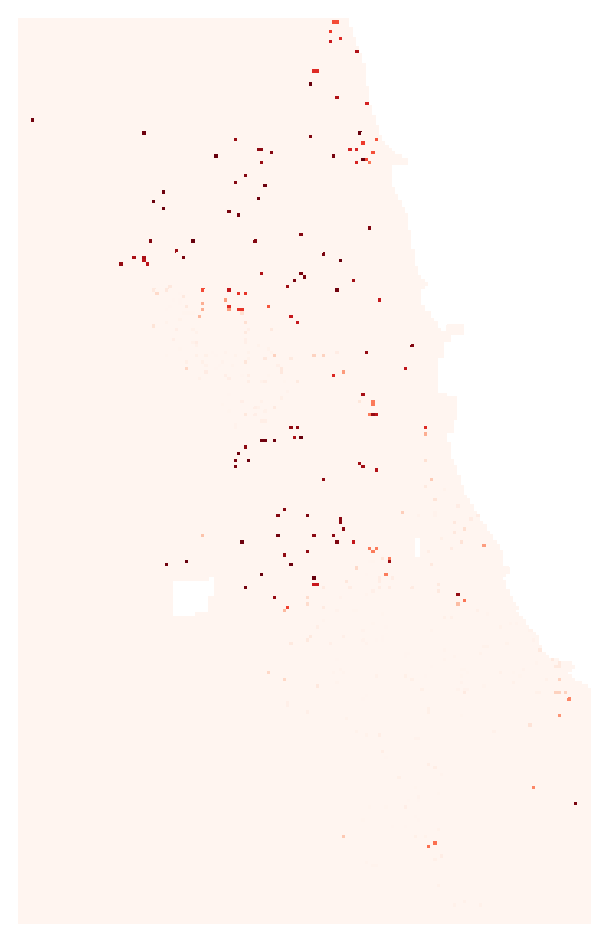
\includegraphics[width=.48\linewidth]{gfx/HeatmapPctWhiteCrime.png}} \\
    \caption{Heatmaps of the "true" $\hat{f}$ values. These maps were produced using \autoref{eq:f_hat1} and \autoref{eq:f_hat2} but with the actual number of crimes in each region as the values of $f$.}
    \label{fig:heatmaps_f_hat}
\end{figure}

Finally, \pp is likely to be less transparent to the police force and the community that they are responsible for than a measure like the naive counting measure. Patrol officers and officials are not likely to understand how and why the model generates its results, since the product is sold to police departments as a black box. Moreover, relying on a third-party vendor to handle predictions runs the risk of feedback loops, as suggested by other researchers \citep{lum_predict_2016,ensign_runaway_2017,ensign_decision_2018}. The devil is in the details when using predictive policing software, and police department ought not treat the results or mechanisms of \pp as infallible.

%************************************************
\chapter{Conclusion}\label{ch:conclusion}
%************************************************

% Reframe the work of this paper in terms of intrinsic accuracy and fairness trade-offs (FairPol doesn't work as well as intended)

To summarize, we implemented an existing predictive policing model and assessed it for accuracy and fairness relative to a baseline measure. We found that the method was not more accurate than the baseline method nor was it fairer. We proposed a post-processing fairness task that seems to improve the fairness of results while maintaining a good amount of accuracy. We also discussed some of the normative implications of this work on the use of predictive policing.

\section{Further Work}
% \begin{itemize}
% \item Extend to multiple races
% \item Replicate tests on other datasets
% \item Replicating FairPol on a dataset that contains race data for individual
% crimes
% \item Moving beyond the "observational" notions of fairness surveyed in this
% paper
% \item Proving the NP-completeness of the fair-ranking problem
% \item Create approximation algorithms for the fair-ranking problem
% \end{itemize}
The knapsack problem and many of its variants, including the multi-dimensional knapsack problem, are known to be NP-hard problems. It might be interesting to prove that the knapsack reduction discussed in \autoref{ch:fairpol} is also NP-hard, despite the fact that there is likely to be correlation between the value of each item and the costs associated with each item.

However, we would also like to suggest future lines of computer science research that more directly promote justice and equity. While there has been a heightened interest in assessing the social impacts of various computational techniques in society, much of the scholarly work from computer scientists has been, unsurprisingly, abstract and reductive. This work has been abstract in the sense that they detach themselves from real-world usage and complexity of algorithmic applications and reductive in the sense that they boil down complex and ambiguous concepts such as "fairness" and "equity" into single and ultimately limited equations. Our hope is that this thesis shows that not all computer scientists have to be bound by the preferences of their field.

For instance, computer scientists can begin to model different response from communities in response to over-policing and how that might change the calculus of a police department (this work would be similar in nature to \citet{liu_delayed_2018}).

Computer scientists could also consider different objective functions other than accuracy for predictive policing algorithm, such as the impact of policing on police-civilian relationships or sentiments of community safety.

Recent research on "dirty data" in predictive policing systems also complicates the results of this paper \citep{richardson_dirty_2019}. The data in criminal justice systems reflect not only incidences of crime, but also policing policy---and bias. Many crimes go unreported or unrecorded in the criminal justice system for a variety of reasons. At other times, false crimes are recorded or the number of crimes are over-reported. It may be worthwhile to study how different kinds of hypothesized systematic bias in data collection change the results of this paper. Essentially, one could conduct a robustness test for the results in this paper by assuming that police data tend to systematically over-sample some regions and under-sample some regions based on demographics (as was the central thesis in \citet{lum_predict_2016}).

Finally, it would be interesting to deploy causal notions of fairness (as opposed to the observational notions discussed in \autoref{ch:fairness_primer}) in the context of predictive policing.
\cleardoublepage
% \ctparttext{You can put some informational part preamble text here.}
% \part{The Showcase}\label{pt:showcase}
%\addtocontents{toc}{\protect\clearpage} % <--- just debug stuff, ignore
%\include{multiToC} % <--- just debug stuff, ignore for your documents
% ********************************************************************
% Backmatter
%*******************************************************
\appendix
%\renewcommand{\thechapter}{\alph{chapter}}
\cleardoublepage
\part*{Appendix}
%********************************************************************
% Appendix
%*******************************************************
% If problems with the headers: get headings in appendix etc. right
%\markboth{\spacedlowsmallcaps{Appendix}}{\spacedlowsmallcaps{Appendix}}
\chapter{HC and LO Usage} \label{app:hc_lo_usage}

% \emph{Note to non-Minervans reading this document: }

\section{HCs}

\newcommand\hashtag{\item[\textbf{\#}]}
\begin{itemize}
\hashtag optimization (FA): Because the parameter space for \pp is non-convex (see \autoref{ch:predpol_primer} for a discussion of each parameter), any given run of the EM algorithm is likely to return a local optimum. Thus, I added multiple restarts with random initial values and chose the set of parameters that produced the highest likelihood of generating the data.

\hashtag simulation (FA): This thesis contains a combination of theory and simulation, with an emphasis on the latter. The post-processing modification task introduced in \autoref{ch:fairpol} may theoretically correspond to satisfying a notion of fairness, but that must be tested on actual data and prediction results. Technically speaking, one can only guarantee fairness at prediction time, in terms of the predicted intensity values. Simulation is required to verify these results in practice.


% \hashtag dataviz (EA): In displaying the curves for fairness (\autoref{fig:fairness}), I had to carefully consider what the fairness measure indicates and how it would be represented on the y-axis. The fairness notion I considered was particularly tricky because...
\hashtag correlation (FA): In several places throughout this text (\autoref{sec:fair_unaware} and \autoref{sec:discussion}), Pearson's r is used as a cheap test for statistical independence, though the two terms are not synonymous. Pearson's r tests for a linear relationship among values and can be fooled by a variety of other types of relationships (such as a parabolic one). Statistical independence, on the other hand, is a more abstract notion that accounts for a variety of dependencies, including linear ones. I chose to use correlation as a indicator for dependence for three reasons. First, in the variables considered, non-linear dependencies would be quite odd and hard to explain (for instance, consider a parabolic relationship between proportion black/white in a grid cell and the number of crimes). Second, testing for conditional independence among continuous variables is a difficult problem. Moreover, the points involving Pearson's r are not the main results of this work (i.e. testing whether \pp satisfies sufficiency and explaining the relationship between predicted intensities and demographics). Further work would be necessary to verify or refute the early results from Pearson's r, but either outcome would not undermine the central theses of this work.

\hashtag modeling (EA): The word "model" has been overloaded; the aims of predictive and descriptive modeling are quite different. My results suggest that \pp may function well as a descriptive model for criminologists and sociologists to examine, but real-world constraints hampers its application to predictive modeling. It is possible to make abstract ML models that perform better than \pp  (e.g. \citet{flaxman_scalable_2018}), but those models have even less descriptive value than \pp (which, all things considered, is not that sophisticated).

% \hashtag decisionselection (EA): Perspective of police department, which decision procedure to use

\hashtag studyreplication (EA): The importance of reproducibility shows up in two places in my thesis. First, I took deliberate steps to make my implementation and simulation code as reproducible as possible. I included download and cleaning scripts for all the data used in this study, and I commented each of my functions as well as my scripts. This document also contains a prose description of the implementation (\autoref{app:methodology}). Second, in \autoref{sec:caveats}, I talk explicitly about the relationship of my work to previous studies on \pp, and suggest ways in which my work might be flawed. Both of these are in the service of fostering open science and communication.

\hashtag purpose (CS), ethicalframing (CS): In this thesis, I took the perspective of agents with potentially conflicting viewpoints: one who only cares about unconstrained accuracy and one who also cares about fairness and justice. I demonstrated that \pp, with regard to either set of motivations, fails to impress. This approach also squares the circle of intuitive tensions between accuracy and fairness in a predictive policing context.

\hashtag multiplecauses (CS), sampling (FA): An unexplored fact of this work is the relationship between bias in crime data and my simulation results (I make mention of this issue in the conclusion). Computer scientists and practitioners have a tendency to treat data as the truth, when in reality, data collection practices are far from guaranteed to be a random sample from the population. In this paper, what has been used as and referred to as "crime data" is actually the result of a system of interactions, only one of which is the true occurrence of criminal activity. Other important aspects of the data generation process include the decision to report some crimes but not others and historical police policies that may distort the picture of crime. There are issues with the Chicago data itself, due to a legacy of biased (both in the statistical and normative sense) policing practices and data entry, that might change how we should interpret the results of a predictive policing algorithm. Understanding the data in this paper as the result of this complex generation mechanism leads to different interpretations of a "predictive policing" algorithm. For example, one such alternative interpretation is that the results in this paper are actually predictive of police activity, and not of crimes themselves. That interpretation of the data suggests further reason to be wary of predictive policing algorithms in general, since the data they are trained on may not actually be usable. It would also be interesting to consider if the data are systematically biased (in terms of sampling) in such a way that undermines a central result of this paper (that \pp does not necessarily predict more accurately than a simple baseline).

% An earlier reviewer of my work brought to my attention the importance of paying attention to data generation mechanisms in any empirical study and particularly for a topic as sensitive as policing, and they have my thanks.

% \hashtag multiplecauses (CS): Crime is a complex phenomenon, so ought we utilize a very assumption-free model like PredPol? The one type of cause used by PredPol (geographic vicinity) is a strong proxy for race.

% \hashtag psychologicalexplanation (CS): The way police officers use a predictive policing tool may be complex? While it's an academic point to say that PP systems predict risk and not certainty, the difference in practice for the police officer might be quite different (fight-or-flight response).

% \hashtag evidencebased (MC):

\hashtag audience (MC): I intend for this paper to appeal to both technical and non-technical audiences. The latter group can just skip over any technical material or formulae, since most of the arguments and contributions of this paper can be explained in non-technical terms. As a point of differentiation from other computer science papers that I have read, I have explicitly included sections which talk about normative and ethical issues, such as the relationship between different notions of fairness (\autoref{ch:fairness_primer}).

% \hashtag cognitivepersuasion, emotionalpersuasion (MC): My thesis conducts what is essentially a cost-benefits analysis for \pp, a strategy which may not be convincing to some audiences based on their political or ideological predispositions. A companion to this document, such as a popular science article explaining its results, could incorporate emotional persuasion by telling stories of how police officers use predictive policing software and how policed communities are affected as a result.

\end{itemize}

\section{LOs}

\begin{itemize}
\hashtag justice (AH164), technicalfairness (Custom): I demonstrate my understanding of both philosophical justice and technical notions of fairness in \autoref{ch:fairness_primer}. The kind of philosophical justice discussed here could be expanded in future work, since I restrict my attention mostly to procedural justice (is the allocation process fair?) rather than substantive justice (is the final standing of each person in society fair?). The lines between these two kinds of fairness do blur. One example of substantive fairness that differs from procedural fairness is to look at the number of people of different races that end up with a criminal record as a result of a predictive policing system. That goal is different from merely demographic parity (that there is no statistical relationship between the people predicted by an algorithm and the person's race). One could have demographic parity and still have unfairness (in the substantive sense) if the later decisions in the criminal justice process affected people of different races differently. Measuring and optimizing for that kind of fairness has not been discussed in this paper.

\hashtag expectationmaximization (CS156): I had to implement and verify an expectation-maximization algorithm to train the internal parameters for \pp; see the above discussion on optimization.

\hashtag probabilitytheory, graphicalmodels (CS146): I applied my knowledge of statistical models to understand and implement \pp. While graphical models did not explicitly factor into this paper, I did draw graphical models for myself as I worked through the papers introducing \pp.

% \hashtag modelmetrics (CS156): 

\hashtag novelapplication (CS110): I proposed how a fairness task could be transformed into a version of a different computational problem, the multi-dimensional knapsack problem (itself a variant of the knapsack problem).
\end{itemize}

\chapter{Supplementary Material} \label{app:math}

\section{Verifying \pp for Sufficiency} \label{sec:sufficiency}
% Reminder to swap out "calibration" for "sufficiency"
% Note: Google testing for conditional independence via correlation tests

Sufficiency requires that conditional on the predicted status, the protected attribute is independent from the true status. In our setting, all three variables (protected attribute, prediction, and true status) are continuous, which complicates both statistical and graphical checks. Statistically, verifying conditional independence for continuous variables is a hard problem \citep{bergsma_testing_2004}. Graphically, \citet{barocas_fairness_2018} introduce the approach of plotting accuracy curves for each predicted group separately. However, because the protected attribute in our case is continuous for each grid cell, this approach also does not work.

To provide initial evidence that \pp satisfies sufficiency, we bin grid cells by predicted intensity and calculate the correlation between number of actual crimes and demographic (percentage black or white) for the grid cells in each bin. Within each bin of cells of similar predicted intensity, we should see no correlation (close to 0.0) between the number of actual crimes and the percentage black/white. We repeat this procedure for each day that was predicted in the test set, and plot each observed correlation as a separate point (so there may be more than one point for the same bin). Not every bin on each day has enough grid cells (more than two) to perform Pearson's r meaningfully; those points are omitted from the graph.

\autoref{fig:sufficiency} shows the scatter plot of these results. If \pp is calibrated, we would expect most of the y-values to be close to zero, which is what we observe. We see instead that for some days, there is indeed a strong correlation between demographics and number of crimes, even after conditioning on predicted intensity. Further research is necessary to verify these results and, if the results are verified, interrogate their implications.
% Results from the same test day in 2015 have the same color. Reassuringly, we do not see any clustering based on color. If we did, we might still be concerned about the calibration of \pp, since on

\begin{figure}[bth]
    \myfloatalign
    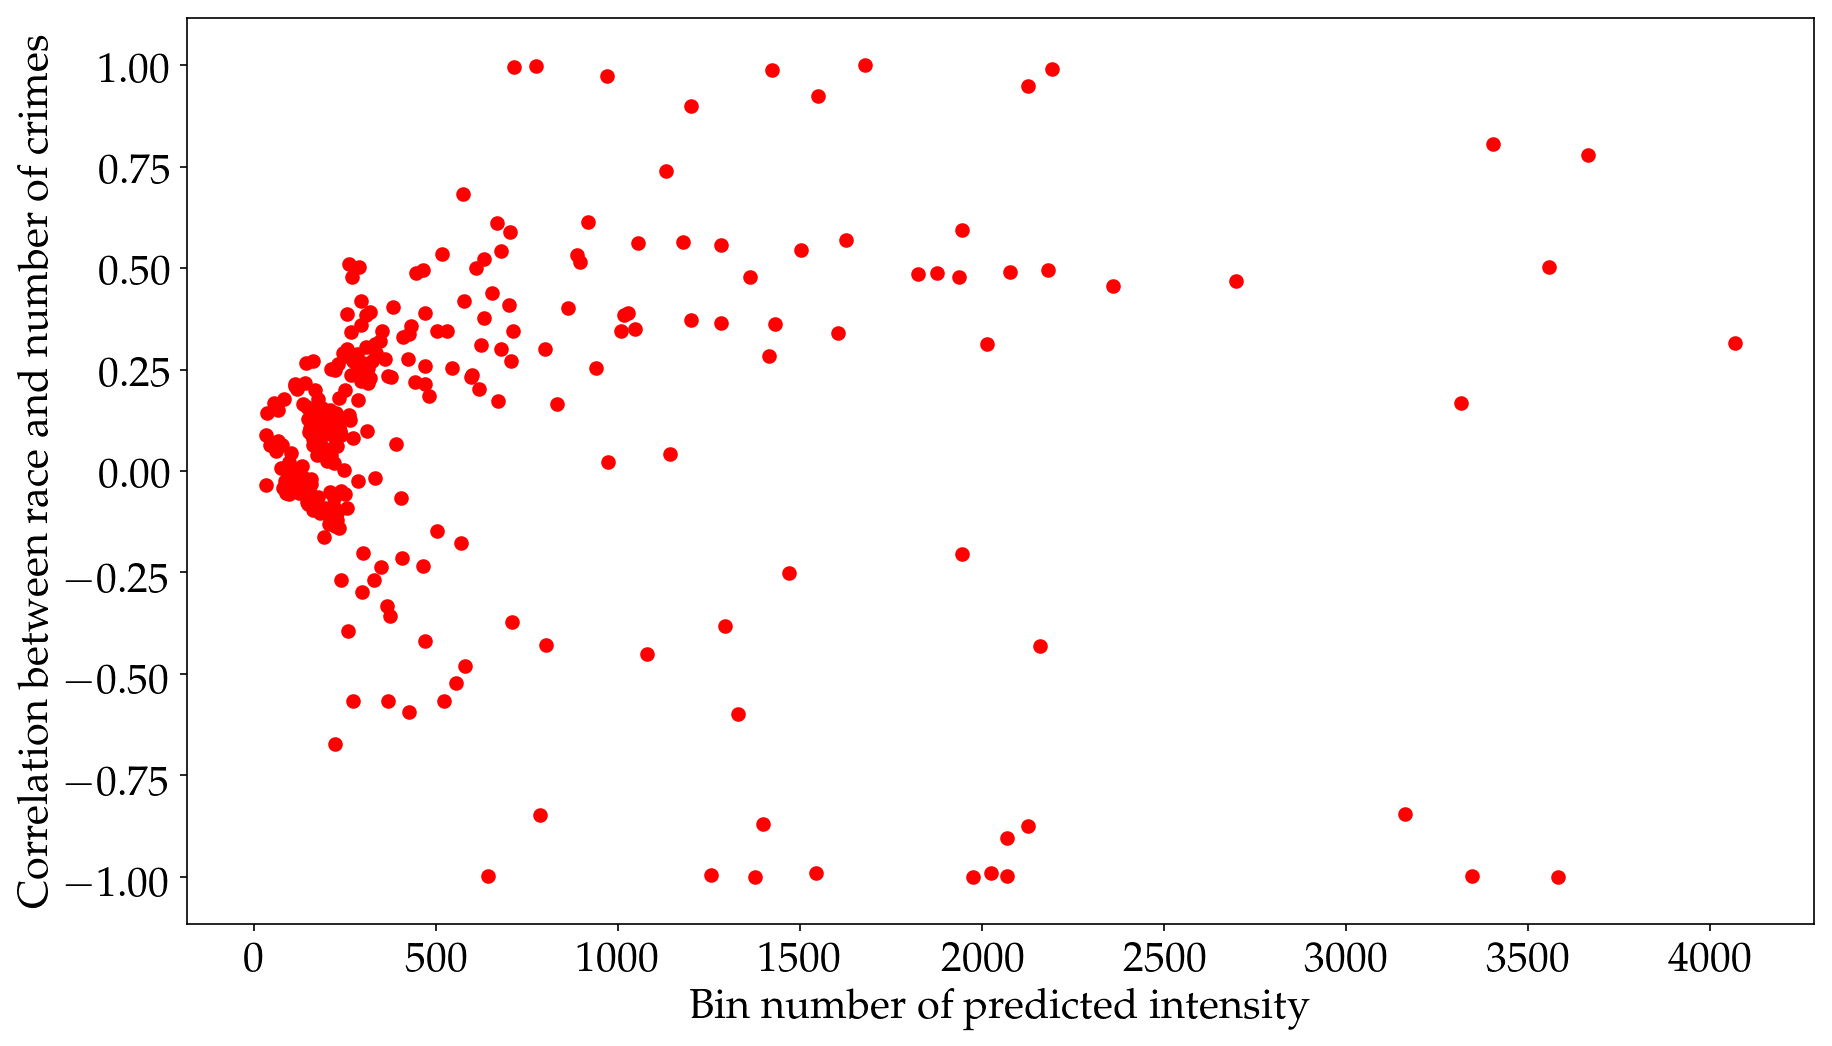
\includegraphics[width=.9\linewidth]{gfx/CalibrationScatter.png}
    \caption{Verifying that \pp satisfies sufficiency}
    \label{fig:sufficiency}
\end{figure}

\pagebreak
\section{Proof of Incompatibility from \autoref{ch:fairness_primer}} \label{proof:ch_3}

The following proves the incompatibility of these two fairness notions in real-world situations:
\begin{align}
\intertext{Equalized Odds:}
p(\hat{Y} \mid Y, A = 1) &= p(\hat{Y} \mid Y, A = 0) \label{eq:eq_op}\\
\intertext{Equal Desert (Sufficiency):}
p(A \mid Y = 1) &= p(A \mid \hat{Y} = 1) \label{eq:def_other1}\\
p(A \mid Y = 0) &= p(A \mid \hat{Y} = 0) \label{eq:def_other2}
\end{align}
Equation~\ref{eq:def_other1} says, "the percentage of crime group $A$ is responsible for equals the percentage of group $A$ in the locations visited." The proof proceeds by showing that if all of the above equations are true, edge-case conditions must also be true (and so in general, not all of the above equations can be true).\footnote{The form of this proof closely resembles the proofs found in \citet{barocas_fairness_2018}.} Start by applying the law of total probability to the right-hand side of equation~\ref{eq:def_other1}.
\begin{align}
p(A \mid \hat{Y} = 1) &= \sum_{Y} p(A \mid Y, \hat{Y} = 1) \; p(Y \mid \hat{Y} = 1) \label{eq:proof_line1}\\
&= \sum_{Y} p(A \mid Y) \; p(Y \mid \hat{Y} = 1)
\end{align}
The second line holds from applying equation~\ref{eq:eq_op}, since the protected category $A$ will be independent from predictions $\hat{Y}$ given the true status $Y$.
\begin{align}
p(A &\mid \hat{Y} = 1)\\
&= p(A \mid Y = 0)p(Y = 0 \mid \hat{Y} = 1) + p(A \mid Y = 1)p(Y = 1 \mid \hat{Y} = 1)\\
&= p(A \mid Y = 0)p(Y = 0 \mid \hat{Y} = 1) + p(A \mid Y = 1)(1 - p(Y = 0 \mid \hat{Y} = 1))\\
&= p(A \mid \hat{Y} = 0)p(Y = 0 \mid \hat{Y} = 1) + p(A \mid \hat{Y} = 1)(1 - p(Y = 0 \mid \hat{Y} = 1))
\end{align}
Here, we make use of the assumptions in equations~\ref{eq:def_other1} and
\ref{eq:def_other2}. Now dividing both sides by $p(A \mid \hat{Y} = 1)$:
\begin{align}
1 &= \frac{p(A \mid \hat{Y} = 0)}{p(A \mid \hat{Y} = 1)}p(Y = 0 \mid \hat{Y} = 1) + 1 - p(Y = 0 \mid \hat{Y} = 1)\\
0 &= p(Y = 0 \mid \hat{Y} = 1) \left(\frac{p(A \mid \hat{Y} = 0)}{p(A \mid \hat{Y} = 1)} - 1\right)
\end{align}
So either $p(Y = 0 \mid \hat{Y} = 1) = 0$ or $p(A \mid \hat{Y} = 0) = p(A \mid
\hat{Y} = 1)$. The first condition states that the algorithm has 100\%
precision. By conditioning on $\hat{Y} = 0$ instead of $\hat{Y} = 1$ in
equation~\ref{eq:proof_line1}, we also obtain the implication that $p(Y = 0
\mid \hat{Y} = 0) = 0$. In other words, this first condition states that the
policing algorithm must be 100\% accurate. The second condition, because of our
assumptions in in equations~\ref{eq:def_other1} and \ref{eq:def_other2}, can
also be rewritten as: $p(A \mid Y = 0) = p(A \mid Y = 1)$. It is rarely the case that the demographics of those who do commit crimes and those who do not are identical however.

Because \autoref{eq:eq_op}, \autoref{eq:def_other1}, and \autoref{eq:def_other2} together imply edge case conditions, we can conclude that in general all three cannot hold simultaneously.

\chapter{Methodology} \label{app:methodology}

This appendix describes the data collection, data cleaning, and simulation process of the present research. It is meant to accompany the code provided at: \url{https://github.com/MWYang/Capstone-FairPol}, and offers a high-level description of the procedure specified in the README there. 

With a fast Internet connection on a MacBook Pro (Retina, 13-inch, Early 2015, 2.7 GHz processor, and 16 GB of RAM), the whole experimental process (downloading the RAW data, processing the data, running the simulation, and collecting results) takes about 4 hours.

\section{Data Collection}

There are three sources of data for the project:
\begin{itemize}
    \item Chicago crime data
    \item 2015 American Community Survey demographics by 2010 Census tracts
    \item 2010 Census Tracts GeoJSON shapefile
\end{itemize}
Download links for all of the data sources can be found in the corresponding scripts in the GitHub repository. The first dataset is used to train \pp and make forecasts, while the remaining two are used to associate each grid cell in the \pp model with demographic information. Downloading demographic information makes use of the Python library \texttt{censusdata}, while the other two are available via public URLs.

\section{Data Processing}

The Chicago data are filtered to only include homicides in the years 2012-2015, inclusive. Rows with missing data in the 'X Coordinate', 'Y Coordinate', 'Latitude', 'Longitude', or 'Date' columns are dropped as these are all features required for simulation.

To prevent overflow errors in the \pp simulation, x- and y-coordinate values are rescaled. The rescaling makes use of longitude and latitude calculations to ensure that 0.01 rescaled units corresponds to 150m, so that the final grid cell size in \pp is 150m $\times$ 150m. Moreover, we also 0-1 normalize the dates in the data to also avoid overflow.

\section{\pp Simulation}

As described in \autoref{ch:predpol_primer}, \pp simulation proceeds by iteration over the set of historical training data. First, \pp learns its internal parameters ($\eta$, $\omega$, and $\sigma$) via an expectation-maximization (EM) procedure. The EM equations are reproduced from \citet{mohler_marked_2014} below. In the E-step, compute two matrices $\mathbf{p}$ and $\mathbf{p^b}$ that indicate the probability of the $i$th event causing the $j$th event. If there are $N$ crimes in the training data, then both these matrices will be $N \times N$ square matrices. The sum of all the values in $\mathbf{p} + \mathbf{p^b}$ also measures the likelihood of the data given the current parameters, which is used to assess the fitness of the parameters across random restarts.
\begin{align}
    p_{ij} &= \frac{
        \omega \exp\left(-\omega(t_j - t_i)\right)
        \frac{1}{2 \pi \omega^2} \exp\left(
            -\frac{(x_j - x_i)^2 + (y_j - y_i)^2}{2\sigma^2}
        \right)
    }{f(x_j, y_j, t_j)}\\
    p^b_{ij} &= \frac{
        \frac{1}{2 \pi \eta^2} \exp\left(
            -\frac{(x_j - x_i)^2 + (y_j - y_i)^2}{2\eta^2}
        \right)
    }{T f(x_j, y_j, t_j)}
\end{align}
$T$ is the length of the time window (the maximum $t$-value, if the minimum value is 0) in the training data. Given the values in the E-step, we update the values of the parameters in the M-step with the following equations:
\begin{align}
    \omega &= \frac{\sum_i \sum_j p_{ij}}{
        \sum_i \sum_j p_{ij} (t_j - t_i) + 
        \sum_i (T - t_i) \exp(-\omega(T - t_i))
    }\\
    \sigma^2 &= \frac{
        \sum_i \sum_j p_{ij} \left(
            (x_j - x_i)^2 + (y_j - y_i)^2
        \right)
    }{2 \sum_i \sum_j p_{ij}}\\
    \eta^2 &= \frac{
        \sum_i \sum_j p^b_{ij} \left(
            (x_j - x_i)^2 + (y_j - y_i)^2
        \right)
    }{2 \sum_i \sum_j p^b_{ij}}
\end{align}
EM proceeds by taking alternate E-step and M-step updates until the parameter values converge.

To make predictions, \pp takes as an input all historical crime data observed up until the day desired for prediction. Predicted intensities are calculated for each grid cell using \autoref{eq:predpol_main} in \autoref{ch:predpol_primer}. The grid cells can then be sorted by the predicted intensity to output a list of predictions. We do so for every day in 2015, using the data from years 2012-2014 and any previously seen days in 2015 to compute intensities. Because this process is fairly time-consuming, we store all of the predicted intensities for each day in 2015 to speed up our fairness modifications.

\section{Fairness Modifications}
Computing the post-processing modification task described in \autoref{ch:fairpol} is relatively straightforward. After computing the $\hat{f}$ values as described in that section, we pass those values as weights to a library for solving the multi-dimensional knapsack problem. To speed up the performance of the library, we restrict the number of items that the knapsack solver receives: if $K$ items are desired ultimately, we take only the top $5K$ items, as ranked by the original \pp intensity. We found experimentally that restricting items in this manner did not impact the ultimate accuracy of the knapsack solver, and instead resulted in a significant boost in runtime. Our function for computing the fairness modification takes in a parameter controlling this restriction, so researchers can experiment with this as well.

% \section{Analysis}

% Generating pseudo-ROC curves
%********************************************************************
% Other Stuff in the Back
%*******************************************************
%%TC:ignore
\cleardoublepage%********************************************************************
% Bibliography
%*******************************************************
% work-around to have small caps also here in the headline
% https://tex.stackexchange.com/questions/188126/wrong-header-in-bibliography-classicthesis
% Thanks to Enrico Gregorio
\defbibheading{bibintoc}[\bibname]{%
  \phantomsection
  \manualmark
  \markboth{\spacedlowsmallcaps{#1}}{\spacedlowsmallcaps{#1}}%
  \addtocontents{toc}{\protect\vspace{\beforebibskip}}%
  \addcontentsline{toc}{chapter}{\tocEntry{#1}}%
  \chapter*{#1}%
}
\printbibliography[heading=bibintoc]

% Old version, will be removed later
% work-around to have small caps also here in the headline
%\manualmark
%\markboth{\spacedlowsmallcaps{\bibname}}{\spacedlowsmallcaps{\bibname}} % work-around to have small caps also
%\phantomsection
%\refstepcounter{dummy}
%\addtocontents{toc}{\protect\vspace{\beforebibskip}} % to have the bib a bit from the rest in the toc
%\addcontentsline{toc}{chapter}{\tocEntry{\bibname}}
%\label{app:bibliography}
%\printbibliography

%%TC:endignore
% \cleardoublepage%*******************************************************
% Declaration
%*******************************************************
\pdfbookmark[0]{Declaration}{declaration}
\chapter*{Declaration}
\thispagestyle{empty}
Put your declaration here.
\bigskip

\noindent\textit{\myLocation, \myTime}

\smallskip

\begin{flushright}
    \begin{tabular}{m{5cm}}
        \\ \hline
        \centering\myName \\
    \end{tabular}
\end{flushright}

% \cleardoublepage\pagestyle{empty}

\hfill

\vfill


\pdfbookmark[0]{Colophon}{colophon}
\section*{Colophon}
This document was typeset using the typographical look-and-feel \texttt{classicthesis} developed by Andr\'e Miede and Ivo Pletikosić.
The style was inspired by Robert Bringhurst's seminal book on typography ``\emph{The Elements of Typographic Style}''.
\texttt{classicthesis} is available for both \LaTeX\ and \mLyX:
\begin{center}
\url{https://bitbucket.org/amiede/classicthesis/}
\end{center}
Happy users of \texttt{classicthesis} usually send a real postcard to the author, a collection of postcards received so far is featured here:
\begin{center}
\url{http://postcards.miede.de/}
\end{center}
Thank you very much for your feedback and contribution.

\bigskip

\noindent\finalVersionString

%Hermann Zapf's \emph{Palatino} and \emph{Euler} type faces (Type~1 PostScript fonts \emph{URW
%Palladio L} and \emph{FPL}) are used. The ``typewriter'' text is typeset in \emph{Bera Mono},
%originally developed by Bitstream, Inc. as ``Bitstream Vera''. (Type~1 PostScript fonts were made
%available by Malte Rosenau and
%Ulrich Dirr.)

%\paragraph{note:} The custom size of the textblock was calculated
%using the directions given by Mr. Bringhurst (pages 26--29 and
%175/176). 10~pt Palatino needs  133.21~pt for the string
%``abcdefghijklmnopqrstuvwxyz''. This yields a good line length between
%24--26~pc (288--312~pt). Using a ``\emph{double square textblock}''
%with a 1:2 ratio this results in a textblock of 312:624~pt (which
%includes the headline in this design). A good alternative would be the
%``\emph{golden section textblock}'' with a ratio of 1:1.62, here
%312:505.44~pt. For comparison, \texttt{DIV9} of the \texttt{typearea}
%package results in a line length of 389~pt (32.4~pc), which is by far
%too long. However, this information will only be of interest for
%hardcore pseudo-typographers like me.%
%
%To make your own calculations, use the following commands and look up
%the corresponding lengths in the book:
%\begin{verbatim}
%    \settowidth{\abcd}{abcdefghijklmnopqrstuvwxyz}
%    \the\abcd\ % prints the value of the length
%\end{verbatim}
%Please see the file \texttt{classicthesis.sty} for some precalculated
%values for Palatino and Minion.
%
%    \settowidth{\abcd}{abcdefghijklmnopqrstuvwxyz}
%    \the\abcd\ % prints the value of the length

% ********************************************************************
% Game Over: Restore, Restart, or Quit?
%*******************************************************
\end{document}
% ********************************************************************
